\chapter{一般图上动态规划的构建}
\label{chap:general-graph-dp-construction}

上一章的四环算例说明，依赖图含环时，消去一个变量会把它的邻居耦合起来，接口必须同时保留多个变量。于是在计算任何数值之前，要先回答：应当把哪些变量放在一起处理，每个子问题以哪些变量为接口，子问题之间按什么次序传递结果，才能保证每个局部项有处可放、每张摘要表不丢失信息？

本章只处理这个结构问题，输入是各局部函数的作用域，输出是一个可以核验的计算结构；具体数值表的计算留给下一章。第~\ref{sec:graph-dp-construction-problem}节写清输出要求，引入袋、接口和树分解，并说明保留变量的查询对结构提出什么额外要求。

随后两节从两个方向构建同一种结构。第~\ref{sec:graph-variable-elimination}节按一个消元次序模拟消元，用填充边记录新产生的耦合，把每一步同时处理的变量连成一棵树；第~\ref{sec:graph-dp-from-decomposition}节从一个给定的树分解出发，证明每个局部项都能放进某个袋、接口确实分隔两侧，并从叶袋读出一个相容的消元次序。

第~\ref{sec:graph-dp-construction-equivalence}节把两个方向合起来：消元得到的中间函数对应袋之间的接口消息，最小诱导宽度等于树宽，并在四环上把双向转换逐步做一遍。第~\ref{sec:graph-tree-decomposition-construction}节讨论怎样实际得到好的结构：贪心选择消元次序、利用弦图的完美消元序、借第~\ref{chap:minimum-spanning-tree}章的最大权生成树构造团树，以及怎样检验构建结果。

本章依赖上一章的消元操作式~\eqref{eq:graph-dp-elimination-step}与四环算例，以及第~\ref{sec:graph-trees-forests}节关于树的基本事实：树中两点之间的路径唯一，选根后每个非根节点有唯一的父节点。

% 第12章第1节：构建问题与输出要求（作用域与依赖图、袋与接口、树分解与树宽、接口与内部变量、保留变量的结构要求）。

\section{构建问题与输出要求}
\label{sec:graph-dp-construction-problem}

第~\ref{sec:graph-dp-construction-goal}小节提出了一般图上动态规划的三项要求：每个局部项有处可放，接口足以概括内部变量，子问题的依赖可以排序。本节把这些要求写成可以核验的定义。先固定构建的输入，再引入袋与接口，用树分解刻画合法的袋树，并说明每个子问题的接口与内部变量；最后说明保留变量的查询对结构提出什么额外要求。

\subsection{作用域与依赖图}
\label{sec:graph-dp-scope-graph}

构建的输入只是变量集合$V$和各局部函数的作用域$S_a$，$a\in A$，不含任何函数值。由它们得到第~\ref{sec:graph-dp-factor-graphs}小节的原始图$\mathcal G=(V,E)$：以全部变量为顶点，两个变量同属某个作用域时连一条边。每个作用域$S_a$在$\mathcal G$中两两相邻。

顶点集取全部变量，包括不出现在任何局部函数中的孤立变量。这样的变量不带来成本，但最优配置仍要给它赋值，计数时也要累计它的全部状态，所以它仍须出现在结构中。四环算例的作用域就是四条边，原始图就是环$1-2-3-4-1$本身；三元作用域例子的原始图有五条边，只缺$\{1,4\}$。

构建只使用作用域，所得结构对作用域相同而数值任意的全部问题都适用。某组特定数值可能恰好使一张中间表还能进一步分解（第~\ref{sec:graph-dp-fill-in}小节给出一例），但构建不利用这种巧合：一般数值下必须保留的耦合，构建时一律保留。数值上的进一步化简要回到函数表本身判断，不属于本章的结构问题。

\subsection{袋与接口}
\label{sec:graph-dp-bags}

回到四环算例。第~\ref{sec:graph-dp-four-cycle}小节的计算先同时看$\{1,2,4\}$，产生以$\{2,4\}$为索引的表$\psi_1$；再同时看$\{2,3,4\}$，读入$\psi_1$完成计算。三元作用域例子也一样：若按次序$(1,4,2,3)$消元，消去$x_1$时要同时处理$\{1\}\cup S_1=\{1,2,3\}$，消去$x_4$时处理$\{2,3,4\}$，随后依次处理$\{2,3\}$和$\{3\}$。

每一步产生的新函数会在后面某一步被用到：$\psi_1$与$\psi_4$都在消去$x_2$时被合并，消去$x_2$得到的新函数在消去$x_3$时被使用。

把每一步同时处理的变量集合看成一个节点，按“新函数交给哪一步使用”连接这些节点，就得到图~\ref{fig:graph-dp-bags-interface}中间的一棵树。这棵树只记录了哪些变量要一起处理、表交给谁，与$\phi_A,\phi_B$的具体数值无关，换一组作用域相同的函数，它照样适用。

准备放进同一张表里同时索引的变量集合称为\term{袋}（bag），可以把它想成计算时一次摆上桌面的变量：对它们的每一种联合取值各记一个数。袋组成的树称为袋树。袋树的节点是计算单元，袋树的边表示两个计算单元之间传递一张表；它与原始图中连接两个变量的边含义不同。不同的袋可以有公共变量，例如$\{1,2,3\}$与$\{2,3,4\}$都含$2,3$。

\begin{figure}[!htb]
  \centering
  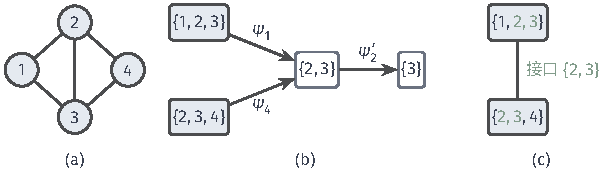
\includegraphics[width=103.283mm]{figures/01-basic-mathematics/04-graphs/tikz/c5-elimination-to-bags/figure.pdf}
  \caption{从消元步骤得到袋。左：三元作用域例子的原始图。中：按次序$(1,4,2,3)$消元时，每一步同时处理的变量集合构成一个袋，箭头表示新函数交给哪一步使用。右：$\{2,3\}$和$\{3\}$已包含在相邻的大袋中，并入后只剩两个袋，它们的交集$\{2,3\}$（绿色）就是接口。}
  \label{fig:graph-dp-bags-interface}
\end{figure}

袋与原始图中的团有关，但不必是团。原始图中两两相邻的顶点集合称为\term{团}（clique）。三元作用域例子中$\{1,2,3\}$是团，$\{1,2,4\}$不是，因为缺边$\{1,4\}$。四环算例中第一个袋$\{1,2,4\}$也不是原始图的团：$2$与$4$在环上不相邻，消去$x_1$后才通过$\psi_1$耦合。所以袋可以重叠，也可以含有原图中不相邻的变量。

\paragraph{接口与一致性}
在三元作用域例子中，袋$\{2,3\}$和$\{3\}$都已包含在相邻的大袋中，可以并入，最后只剩两个袋$\{1,2,3\}$与$\{2,3,4\}$，如图~\ref{fig:graph-dp-bags-interface}右侧。相邻两袋的交集称为它们的接口，这里是$\{2,3\}$；四环算例中两个袋的接口是$\{2,4\}$。这与第~\ref{sec:graph-dp-tree-idea}小节的接口变量含义相同，只是现在接口可以含多个变量。

接口上的变量在两个袋里是同一个变量，不是两个副本。左袋在汇总$x_1$时必须对$(x_2,x_3)$的每种取值分别给出结果，右袋使用这些结果时也必须按同样的$(x_2,x_3)$取值来读。左袋交出的正是一张以接口为索引的表。

两个袋之间只交换这样一张表，所以一个变量的取值也只能经接口从一个袋传到另一个袋，这就限制了袋的连接方式。若某个变量出现在两个不相邻的袋中，而连接它们的袋树路径上有某个袋不含这个变量，那么那个袋发出和收到的表都不以这个变量为索引，两侧便无法约定它取同一个值。另外，袋还必须能容纳所有局部函数，否则有的成本项无处计算。这两项要求合起来，就是下面的定义。

\subsection{树分解与树宽}
\label{sec:graph-tree-decomposition}
\label{sec:graph-dp-decomposition-definition}

在结构上，容纳局部函数的要求落实为每个变量和原始图的每条边都被某个袋包含；保持一致的要求就是上面的连接要求。

\begin{definition}[树分解]
\label{def:graph-dp-tree-decomposition}
设$\mathcal G=(V,E)$是有限无向图。$\mathcal G$的一个\term{树分解}（tree decomposition）由一棵有限树$\mathcal T$（节点集记为$T$）和每个节点$t\in T$上的子集$B_t\subseteq V$组成，满足：
\begin{enumerate}
  \item 顶点覆盖：每个顶点$v\in V$至少属于一个袋；
  \item 边覆盖：对每条边$\{u,v\}\in E$，存在某个袋同时含有$u$与$v$；
  \item 运行交集：对每个顶点$v\in V$，含$v$的节点集合$T_v=\{t\in T:v\in B_t\}$在$\mathcal T$中连通。
\end{enumerate}
第三个条件称为\term{运行交集性质}（running intersection property）。
\end{definition}

运行交集等价于：若$v$同时属于$B_s$和$B_t$，则$\mathcal T$中从$s$到$t$的路径上每个袋都含$v$。因为树中两点之间只有一条路径，$T_v$连通恰好意味着这条路径留在$T_v$中。直观地说，每个变量在袋树上占据一块连成一片的地盘；沿袋树行走，一个变量一旦离开就不会再出现。

\paragraph{梯子形图的分解}
图~\ref{fig:graph-dp-ladder-decomposition}中的梯子形图有两排顶点$1,2,3$与$4,5,6$，每排相邻顶点之间和同一列的两个顶点之间各有一条边。四个袋$\{1,2,4\},\allowbreak\{2,4,5\},\allowbreak\{2,3,5\},\allowbreak\{3,5,6\}$连成一条路径。

可以逐条核对定义。每个顶点都在某个袋中；七条边中，$\{1,2\},\{1,4\}$在第一个袋，$\{4,5\},\{2,5\}$在第二个袋，$\{2,3\}$在第三个袋，$\{5,6\},\{3,6\}$在第四个袋。

再看运行交集：含$2$的袋是前三个，含$5$的是后三个，含$4$的是前两个，含$3$的是后两个，都连成一段。

这个分解像一个窄窗口从左向右扫过梯子：每个袋是窗口某一时刻看到的顶点，相邻两袋的接口是窗口移动时必须记住的顶点。从第一个袋移到第二个袋时，$1$已经处理完毕，可以忘掉，只需记住$\{2,4\}$；之后$4$也处理完毕，只需记住$\{2,5\}$。运行交集保证被忘掉的顶点不会在后面的袋里再次出现，否则它的取值早已无从查找。梯子再长，窗口也只需同时看三个顶点；第~\ref{sec:graph-dp-chain}小节的链上递推是同样的扫描，只是每次只需记住一个变量。

\begin{figure}[!htb]
  \centering
  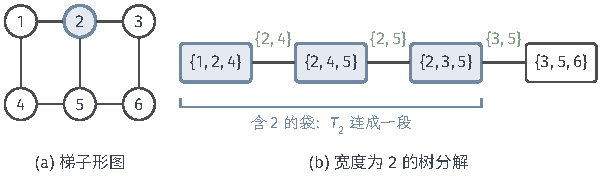
\includegraphics[width=101.85mm]{figures/01-basic-mathematics/04-graphs/tikz/c5-ladder-decomposition/figure.pdf}
  \caption{梯子形图的树分解。(a)两排顶点由三条横档相连。(b)四个袋连成一条路径，像窗口自左向右扫过梯子；边上的绿色集合是相邻两袋的接口，即窗口移动时要记住的顶点。蓝色的袋都含顶点$2$，它们连成一段，满足运行交集。}
  \label{fig:graph-dp-ladder-decomposition}
\end{figure}

\paragraph{运行交集的作用}
只覆盖顶点和边还不够。图~\ref{fig:graph-dp-running-intersection}比较路径$1-2-3-4$上的两种袋连接。两种连接使用同样的三个袋$\{1,2\},\allowbreak\{2,3\},\allowbreak\{3,4\}$，都覆盖了全部顶点和边。

上面一种按$\{1,2\}-\{2,3\}-\{3,4\}$连接，含$2$的两个袋相邻，含$3$的两个袋也相邻，是树分解。下面一种按$\{1,2\}-\{3,4\}-\{2,3\}$连接，含$2$的两个袋被不含$2$的袋$\{3,4\}$隔开。若沿这棵树计算，左端的袋可以选$x_2=0$，右端的袋可以选$x_2=1$，中间的袋不记录$x_2$，无从发现矛盾；拼起来的结果不对应任何一个配置。

\begin{figure}[!htb]
  \centering
  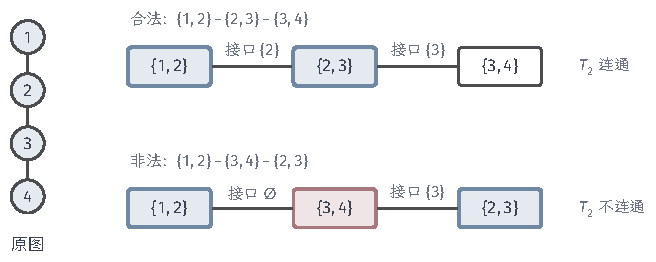
\includegraphics[width=111.016mm]{figures/01-basic-mathematics/04-graphs/tikz/c5-running-intersection/figure.pdf}
  \caption{路径$1-2-3-4$上的合法与非法袋连接。两种连接使用相同的三个袋，都覆盖全部顶点和边。上：含$2$的袋（蓝色）彼此相邻，含$3$的袋也相邻，满足运行交集。下：含$2$的两个袋之间隔着不含$2$的袋$\{3,4\}$（红色），$T_2$不连通，不是树分解。}
  \label{fig:graph-dp-running-intersection}
\end{figure}

\paragraph{宽度与树宽}
\label{sec:graph-dp-treewidth}
袋越大，袋表越大。为了用一个数概括一次分解的规模，定义树分解的宽度为
\[
\max_{t\in T}|B_t|-1,
\]
即最大袋的大小减一；图$\mathcal G$的\term{树宽}（treewidth）是它的全部树分解宽度的最小值，记为$\operatorname{tw}(\mathcal G)$。减一是一种约定，使得至少含一条边的树宽度恰为一。

把整个图放进一个袋总是合法的树分解，宽度为$|V|-1$，所以树宽总有定义，问题在于能否用更小的袋。直观地说，树宽回答的是：把这个图压成一棵树的形状时，每个树节点至少要装下多少个顶点。图越像树，需要的袋越小。

确定一个图的树宽需要两步：构造一个分解给出上界，再证明不存在更小宽度的分解给出下界。下面先给出几个小图的上界构造，图~\ref{fig:graph-dp-treewidth-examples}画出了相应的分解；下界的证明要用到第~\ref{sec:graph-dp-clique-containment}小节的团容纳引理，在那里补上。

单个顶点的图只需一个袋$\{1\}$，宽度为$0$，任何没有边的图都如此。至少含一条边的树有宽度为$1$的分解：任选根$\rho$，为每个非根顶点$u$建袋$\{u,p(u)\}$，其中$p(u)$是父点；若$p(u)$不是根，就把这个袋连到$p(u)$自己的袋上，根的各子点的袋则依次连成一条链。这样，非根顶点$v$出现在自己的袋和各子点的袋中，后者都与前者相邻；根只出现在各子点的袋中，它们连成链，所以运行交集成立。

四个顶点的环$1-2-3-4-1$有宽度为$2$的分解：两个袋$\{1,2,3\}$与$\{1,3,4\}$以一条边相连，接口为$\{1,3\}$；四环算例使用的$\{1,2,4\}$与$\{2,3,4\}$也是一个宽度为$2$的分解，接口为$\{2,4\}$。图~\ref{fig:graph-dp-ladder-decomposition}的梯子有宽度为$2$的分解。四个顶点两两相邻的完全图只用一个袋$\{1,2,3,4\}$，宽度为$3$。

\begin{figure}[!htb]
  \centering
  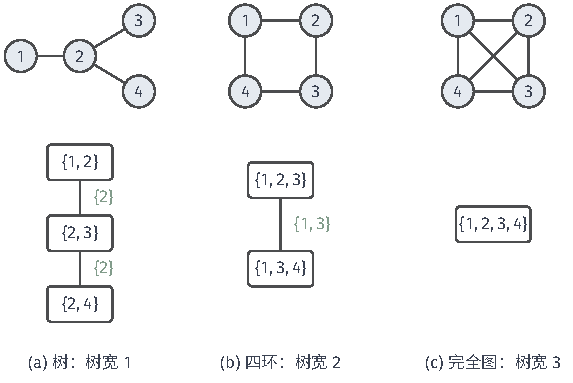
\includegraphics[width=96.95mm]{figures/01-basic-mathematics/04-graphs/tikz/c5-treewidth-examples/figure.pdf}
  \caption{三个四顶点图及其宽度最小的树分解，绿色集合是接口。(a)树：每条边一个袋，宽度为$1$。(b)四环：任何分解都有一个袋含三个顶点，宽度为$2$。(c)完全图：全部顶点必须同在一个袋中，宽度为$3$。}
  \label{fig:graph-dp-treewidth-examples}
\end{figure}

某一次构造得到宽度$k$，只说明$\operatorname{tw}(\mathcal G)\leq k$；要断言树宽恰为$k$，还需要证明不存在更小宽度的分解。

若每个变量至多有$q$个状态，宽度为$k$的分解中，每个袋至多有$k+1$个变量，稠密存储的袋表至多$q^{k+1}$项。这是第~\ref{chap:general-graph-dp-computation}章中主要的枚举规模。实际的总开销还包括袋的个数、接口的大小和每次读取局部函数的成本，宽度只控制其中随状态数指数增长的那一部分，第~\ref{sec:graph-dp-computation-cost}节再作完整分析。

寻找树宽最小的分解与使用一个已经给定的分解是两项不同的任务。前者在一般图上是困难的组合问题；后者只需按定义核验三个条件，再沿树计算。第~\ref{sec:graph-tree-decomposition-construction}节给出的构造方法都只保证得到合法的分解和宽度上界。

\subsection{接口与内部变量}
\label{sec:graph-dp-interface-internal}

一个树分解还要选定根，才能确定子问题的依赖次序。设已给袋树选根$r$，每个非根节点$u$有父节点$p(u)$。称
\[
S_u=B_u\cap B_{p(u)}
\]
为$u$的接口，$I_u=B_u\setminus S_u$为$u$的\term{内部变量}（internal variable）。根没有父节点，约定$S_r=\varnothing$、$I_r=B_r$。

节点$u$对应的子问题是：固定接口取值$\bm x_{S_u}$，汇总内部变量$\bm x_{I_u}$以及$u$下方各子问题已经汇总的内容，输出一张以$\bm x_{S_u}$为索引的表，交给父节点。接口为空时，这张表只有一项，是一个数。四环算例以$\{2,3,4\}$为根时，子节点$\{1,2,4\}$的接口为$\{2,4\}$，内部变量为$\{1\}$；根的内部变量为$\{2,3,4\}$。

为了让每个变量恰好被汇总一次，每个变量应当恰好是一个节点的内部变量。下面的引理说明运行交集保证了这一点，并指出是哪个节点。

\begin{lemma}[每个变量恰在一个袋中作内部变量]
\label{lem:graph-dp-unique-internal}
设$(\mathcal T,\{B_t\}_{t\in T})$是$\mathcal G$的树分解，袋树以$r$为根。对每个$v\in V$，$T_v$中有唯一一个离根最近的节点，记为$\operatorname{top}(v)$，$T_v$的每个节点都是它的后代（含它本身）；并且$v\in I_u$当且仅当$u=\operatorname{top}(v)$。
\end{lemma}

\begin{proof}
由顶点覆盖，$T_v$非空。取$T_v$中深度最小的一个节点$t$。若$y\in T_v$不是$t$的后代，从$y$到$t$的树上路径要先向上经过$y$与$t$的最近公共祖先$z$，而$z$比$t$更靠近根；由$T_v$连通，这条路径留在$T_v$中，于是$z\in T_v$，与$t$的选取矛盾。所以$T_v$的节点都是$t$的后代，深度最小的节点也只有$t$一个，记$\operatorname{top}(v)=t$。

若$u=\operatorname{top}(v)$是根，则$v\in B_r=I_r$。若它不是根，其父节点不是它的后代，因而不在$T_v$中，即$v\notin B_{p(u)}$，所以$v\in I_u$。反过来，若$u\in T_v$而$u\neq\operatorname{top}(v)$，则$u$是$\operatorname{top}(v)$的真后代，从$u$到$\operatorname{top}(v)$的路径第一步就到达$p(u)$；由运行交集，$p(u)\in T_v$，所以$v\in S_u$，不是$u$的内部变量。
\end{proof}

由此，构建的结果应当记录每个节点的袋$B_u$、父节点$p(u)$、接口$S_u$和内部变量$I_u$。这些都是结构信息；节点上要汇总哪些局部函数、汇总出的表取什么值，在第~\ref{chap:general-graph-dp-computation}章求值时确定。

\subsection{保留变量的结构要求}
\label{sec:graph-dp-query-structure}

第~\ref{sec:graph-dp-problem}小节的另一种输出是保留集$R\subseteq V$上的条件最小成本表$F_R(\bm x_R)$。这张表以$\bm x_R$的联合取值为索引，所以必须有某个计算单元同时看到$R$中的全部变量，并且在那之前不能把$R$中的任何变量汇总掉。

结构上采用两条要求。第一，在原始图中把$R$补成团，即在$R$的任意两个不相邻的变量之间加边，得到图$\mathcal G_R$，再为$\mathcal G_R$构建结构。第二，选取的根袋包含$R$。由第~\ref{sec:graph-dp-clique-containment}小节的团容纳引理，$\mathcal G_R$的任一树分解都有某个袋包含$R$，可以选它作根。

根袋包含$R$以后，$R$中每个变量$v$的$\operatorname{top}(v)$都是根，由引理~\ref{lem:graph-dp-unique-internal}，它们不会成为任何非根节点的内部变量，因而不会提前被汇总。根处只汇总$B_r\setminus R$，留下以$\bm x_R$为索引的表。用变量消元描述时，这相当于只消去$V\setminus R$中的变量，最后保留$R$（第~\ref{sec:graph-dp-order-to-decomposition}小节）。

补边可能增大宽度。路径$1-2-3$的树宽为$1$，若$R=\{1,3\}$，补边后得到三角形，树宽变为$2$。所以带保留变量的任务，其宽度要按$\mathcal G_R$计算，不能直接沿用不带查询时的最小树宽；输出表本身还有$\prod_{i\in R}|\mathcal X_i|$项。

在四环算例中取$R=\{1,3\}$。$1$与$3$在环上不相邻，补边$\{1,3\}$后，$\{1,2,3\},\{1,3,4\}$构成宽度为$2$的分解，两个袋都含$R$，任选一个作根即可。原来使用的分解$\{1,2,4\}-\{2,3,4\}$则没有袋同时含$1$和$3$，不能直接回答这个查询。

两个边界情形是：$R=\varnothing$时不加任何要求；$R=V$时$\mathcal G_R$是完全图，任何分解都有一个袋含全部变量，宽度为$n-1$，这与输出表本身就要列出全部配置一致。

% 第12章第2节：由变量消元构建动态规划（消元次序与填充图、消元簇与中间作用域、消元森林的构造、从消元簇得到树分解）。

\section{由变量消元构建动态规划}
\label{sec:graph-variable-elimination}

第~\ref{sec:graph-dp-cycle-interface}小节的消元操作每一步都产生一个新函数，它的作用域由当前所有含该变量的函数共同决定。本节说明，这些作用域可以只在原始图上模拟消元就预先算出，不需要任何函数值。按一个次序模拟一遍，就得到每一步同时处理的变量组和新函数交给哪一步使用，把它们连起来就是一个树分解。

\subsection{消元次序与填充图}
\label{sec:graph-dp-fill-in}

变量消元需要事先给定一个\term{消元次序}（elimination order）$\pi$，即全部要消去的变量的一个排列。消去一个变量时，新函数$\psi_i$的作用域$S_i$由所有含$i$的函数共同决定。在原始图上看，$S_i$恰好是$i$在当前原始图中的邻居集合，因为两个变量相邻当且仅当它们同在某个当前函数的作用域中。新函数读取这些邻居的联合取值，所以消元后的原始图中，这些邻居两两相邻。

\paragraph{一次消元的图操作}
在三元作用域例子中先消去$x_2$，就能看到这一点。$\phi_A$与$\phi_B$都含$2$，$S_2=\{1,3\}\cup\{3,4\}=\{1,3,4\}$，新函数
\[
\psi_2(x_1,x_3,x_4)=\min_{x_2}\bigl[\phi_A(x_1,x_2,x_3)+\phi_B(x_2,x_3,x_4)\bigr]
\]
同时读取$x_1,x_3,x_4$。按$(x_1,x_3,x_4)$的字典序，它的八个值为
\[
\psi_2=(3,\,2,\,0,\,+\infty,\,2,\,1,\,2,\,4),
\]
例如$(x_1,x_3,x_4)=(0,0,0)$处的两个候选为
\[
\phi_A(000)+\phi_B(000)=3,\qquad \phi_A(010)+\phi_B(100)=+\infty.
\]

原始图中原来没有边$\{1,4\}$，消元后必须补上，如图~\ref{fig:graph-dp-elimination-step}所示。这样为记录新函数的联合依赖而补入的边称为\term{填充边}（fill-in edge）。

填充边不表示原问题增加了约束，而是把原来经过$x_2$的间接联系直接记下来。看$x_3=1$的情形：$x_1=0$时，$\phi_A(0,1,1)=+\infty$迫使$x_2=0$，而$\phi_B(0,1,1)=+\infty$又禁止$x_4=1$；$x_1=1$时$x_2$可以取$1$，$x_4=1$仍然可行。原问题中$x_1$通过$x_2$牵制$x_4$。

消去$x_2$以后，这种牵制只能由$\psi_2$自己记录：上面的值中$\psi_2(0,1,1)=+\infty$，而$\psi_2(0,1,0)=0$、$\psi_2(1,1,1)=4$都有限。

若$\psi_2$能拆成一个$(x_1,x_3)$的函数与一个$(x_3,x_4)$的函数之和，固定$x_3=1$后就有
\[
\psi_2(x_1,1,x_4)=g(x_1)+h(x_4).
\]
由$g(0)+h(1)=+\infty$知$g(0)$或$h(1)$为$+\infty$，与$g(0)+h(0)$、$g(1)+h(1)$都有限矛盾。所以这张表必须同时以$x_1$和$x_4$为索引，填充边$\{1,4\}$反映的正是这一点。四环算例中消去$x_1$补入的边$\{2,4\}$也是如此（第~\ref{sec:graph-dp-four-cycle}小节）。

\begin{figure}[!htb]
  \centering
  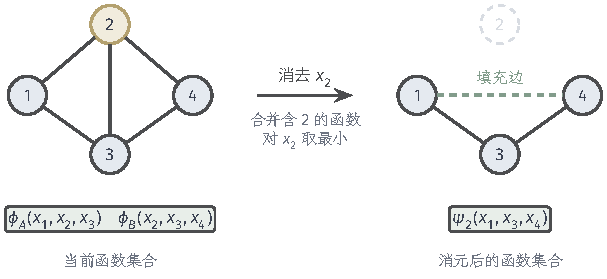
\includegraphics[width=102.687mm]{figures/01-basic-mathematics/04-graphs/tikz/c5-elimination-step/figure.pdf}
  \caption{消去$x_2$时的函数更新与图更新。左：消元前，黄色的$x_2$同时属于$\phi_A$与$\phi_B$的作用域，它的邻居是$1,3,4$。右：消元后，两个函数被新函数$\psi_2(x_1,x_3,x_4)$取代，$x_2$及其关联边被删除，邻居$1,3,4$两两相邻，其中绿色虚线$\{1,4\}$是填充边。}
  \label{fig:graph-dp-elimination-step}
\end{figure}

一般地，消元在原始图上对应一个纯粹的结构操作：把$i$的当前邻居两两连边，然后删去$i$及其关联边。不含$i$的函数提供的边保持不变；含$i$的函数在剩余变量之间提供的边都落在$S_i$内，已被补成的团覆盖；新函数$\psi_i$提供的边恰是$S_i$内的全部点对。因此，消元后函数集合的原始图恰好是对原始图执行这一操作的结果。对消元步数归纳，每一步的当前图都是当前函数集合的原始图，于是只看这个图操作，就能在不计算任何数值的情况下预先知道每一步的$S_i$。

\paragraph{填充图}
按次序$\pi$执行全部消元步骤，把途中补入的所有填充边加入原始图，得到的图称为$\pi$的\term{填充图}（filled graph），记为$\mathcal G^+_\pi$。它记录了这次消元中出现过的全部耦合：原始边来自局部函数，填充边来自中间函数。四环算例按次序$(1,2,3,4)$消元时只补入$\{2,4\}$，填充图是环加上弦$\{2,4\}$。第~\ref{sec:graph-dp-chordal}小节会说明填充图总是弦图。

\paragraph{作用域的结构上界}
图操作只预测新函数可能同时读取哪些变量，不计算新函数的取值，而对特殊的局部函数，新函数可能仍能进一步分解。例如，若$\phi_A(x_1,x_2,x_3)=g(x_1)+h(x_2,x_3)$，则
\[
\psi_2(x_1,x_3,x_4)=g(x_1)+\min_{x_2}\bigl[h(x_2,x_3)+\phi_B(x_2,x_3,x_4)\bigr],
\]
它是一个$x_1$的函数与一个$(x_3,x_4)$的函数之和，实际上并不需要同时索引$x_1$与$x_4$。但这时$\phi_A$本可以作为两个作用域更小的局部函数输入；只给作用域$\{1,2,3\}$时，填充边不知道这种数值巧合。所以补边图给出的是作用域给定、数值任意时新函数作用域的上界；第~\ref{sec:graph-dp-scope-graph}小节说过，构建只依据作用域，不利用这类数值上的巧合。

\subsection{消元簇与中间作用域}
\label{sec:graph-dp-elimination-clusters}

设消元次序为$\pi=(v_1,\ldots,v_n)$。消去$v_i$时，记它在当前图中的邻居集合为$S_i$，也记作$N^+_\pi(v_i)$；上标$+$表示这些邻居都排在$v_i$之后，因为排在前面的顶点已从当前图中删去。称
\[
B_i=\{v_i\}\cup S_i
\]
为第$i$步的\term{消元簇}（elimination cluster）；以顶点本身作下标时，也写作$B_{v_i}$、$S_{v_i}$。它是这一步同时处理的全部变量：计算新函数$\psi_i$要枚举$\bm x_{B_i}$的全部取值，而$\psi_i$的作用域是$S_i$。

消元簇有两条结构性质。第一，$B_i$在填充图中是团：$S_i$在第$i$步被补成团，$v_i$与$S_i$中每个顶点相邻。第二，原始图中排在$v_i$之后的邻居都在$S_i$中，因为在处理$v_i$之前只删去过已处理的顶点及其关联边。

消元次序$\pi$下的最大剩余邻居数$\max_i|S_i|$称为$\pi$的\term{诱导宽度}（induced width），它等于最大消元簇的大小减一。诱导宽度决定了这次消元中最多同时处理多少个变量。

在四环算例中按$(1,2,3,4)$消元：消去$1$时$S_1=\{2,4\}$，补入$\{2,4\}$，消元簇为$\{1,2,4\}$；消去$2$时当前邻居为$\{3,4\}$，其中$4$来自刚补入的填充边，消元簇为$\{2,3,4\}$；随后依次得到$\{3,4\}$和$\{4\}$。诱导宽度为$2$。

三元作用域例子按$(1,4,2,3)$消元，消元簇依次为
\[
 \{1,2,3\},\qquad \{2,3,4\},\qquad \{2,3\},\qquad \{3\},
\]
诱导宽度也是$2$。

\subsection{消元森林的构造}
\label{sec:graph-dp-order-to-decomposition}

\subsubsection{问题与思路}

输入是非空有限无向图$\mathcal G=(V,E)$（通常是局部函数的原始图）和一个消元次序；若有保留集$R$，图取补边后的$\mathcal G_R$，次序只排列$V\setminus R$。要求输出一个树分解，其袋是各步的消元簇，宽度等于诱导宽度。

第~\ref{sec:graph-dp-bags}小节已经从消元步骤读出过袋，这里把那个做法变成算法。消去$v_i$时同时处理的变量构成袋$B_i$。新函数$\psi_i$的作用域是$S_i$，它要等到$S_i$中第一个被消去的变量才会被用到，所以$B_i$应当连到那个变量的袋上。这正是图~\ref{fig:graph-dp-bags-interface}中按“新函数交给哪一步使用”连接袋的做法。

\paragraph{父袋容纳剩余作用域}
这种连接之所以合适，是因为父袋装得下整个$S_i$。设$v_j$是$S_i$中最早被消去的变量。第$i$步把$S_i$补成团；此后直到处理$v_j$之前，$S_i$中没有顶点被删去，因为它们都不早于$v_j$。所以处理$v_j$时，$S_i\setminus\{v_j\}$中的顶点都是$v_j$的当前邻居，即$S_i\setminus\{v_j\}\subseteq S_j$，从而
\[
S_i\subseteq B_j .
\]
也就是说，$\psi_i$交给的那一步恰好会枚举$\psi_i$所需的全部变量。

\paragraph{保留变量与分量}
有保留集$R$时，$R$中的变量不被消去，所有袋最后汇到一个根袋$B_R=R$。若$S_i$含待消去的变量，父袋仍取其中最早被消去者的袋，上面的论证不变，因为$R$中的变量从不删除。若$S_i$非空且全在$R$内，$\psi_i$只读取保留变量，就把$B_i$连到根袋$B_R$。

若$S_i=\varnothing$，$\psi_i$是一个常数，$B_i$没有父袋，成为一个分量的根。原图不连通时会出现多个这样的根；再用任意边把这些根（以及根袋$B_R$，若有）连成一棵树，这些边的接口为空，只用来把各分量的常数汇总起来。

\subsubsection{算法实现}

原图和次序在运行中不变；事先为每个顶点记下它在次序中的位置，以便比较先后。算法维护三项状态：
\begin{itemize}
  \item 当前图$\mathcal H$：用邻接集合存储，初值为$\mathcal G$（有保留集时为$\mathcal G_R$）的副本；
  \item 袋表：为每个已处理的顶点$v$记录袋$B_v$，初值为空；
  \item 父袋表：为每个袋记录它在袋树中的父袋，初值为空。
\end{itemize}
按次序逐个处理顶点，处理$v$时依次做四件事：
\begin{itemize}
  \item 读邻居：读出$v$在当前图$\mathcal H$中的邻居集合$N^+_\pi(v)$；
  \item 记袋：记录$B_v=\{v\}\cup N^+_\pi(v)$；
  \item 补团：把$N^+_\pi(v)$中尚不相邻的顶点两两连边，这些边就是填充边；
  \item 删点：从$\mathcal H$中删去$v$及其关联边。
\end{itemize}
这正是第~\ref{sec:graph-dp-fill-in}小节中消元在原始图上的结构操作。关键在于每一轮都要从更新后的图读取邻居，而不是从原图读取。全部待消去的顶点处理完后，再连接袋：
\begin{itemize}
  \item 对每个$N^+_\pi(v)$含待消去顶点的$v$，令$p(v)$为其中在次序里最早的顶点，把$B_{p(v)}$记为$B_v$的父袋；
  \item 对每个$N^+_\pi(v)$非空且包含于$R$的$v$，把根袋$B_R$记为父袋；
  \item $N^+_\pi(v)$为空的袋没有父袋，作为分量的根；若有多个根（连同$B_R$），用任意边把它们连成一棵树，这些边的接口为空。
\end{itemize}
不加空接口边时，这些袋和父袋连接按分量组成一片森林，称为$\pi$的\term{消元森林}（elimination forest）；加上空接口边后，它成为一棵袋树。

\begin{algorithm}[由消元次序构造树分解]
\label{alg:graph-dp-order-to-decomposition}
输入：非空有限无向图$\mathcal G$，可选的保留集$R$，以及$V\setminus R$的一个消元次序$\pi$。输出：$\mathcal G_R$的树分解，有保留集时根袋为$R$。
\begin{enumerate}
  \item 令$\mathcal H$为$\mathcal G_R$的副本（$R=\varnothing$时即$\mathcal G$），记下每个顶点在$\pi$中的位置。
  \item 按$\pi$依次取顶点$v$：读出$v$在$\mathcal H$中的邻居集合$N^+_\pi(v)$，记录$B_v=\{v\}\cup N^+_\pi(v)$；把$N^+_\pi(v)$中不相邻的顶点两两连边；从$\mathcal H$中删去$v$。
  \item 若$R\neq\varnothing$，建立根袋$B_R=R$。
  \item 对每个$v$：若$N^+_\pi(v)$含待消去的顶点，取其中位置最早的$p(v)$，连接$B_v$与$B_{p(v)}$；若$N^+_\pi(v)$非空且包含于$R$，连接$B_v$与$B_R$；若$N^+_\pi(v)=\varnothing$，$B_v$作为一个根。
  \item 若有多个根（连同$B_R$），用任意边把它们连成一棵树。
\end{enumerate}
\end{algorithm}

\paragraph{执行过程}
图~\ref{fig:graph-dp-elimination-to-decomposition}的例子有边$\{1,2\},\allowbreak\{1,4\},\allowbreak\{2,3\},\allowbreak\{3,4\},\allowbreak\{3,5\},\allowbreak\{4,5\}$，不保留变量，次序为$(1,2,5,3,4)$，表~\ref{tab:graph-dp-decomposition-trace}逐轮列出状态的变化。
\begin{itemize}
  \item 处理$1$：邻居为$\{2,4\}$，二者不相邻，补入填充边$\{2,4\}$，袋为$\{1,2,4\}$。
  \item 处理$2$：当前邻居$\{3,4\}$中的$4$来自上一轮补入的填充边，袋为$\{2,3,4\}$。若误从原图读取，袋就成了$\{2,3\}$，漏掉了消去$x_1$后新函数同时读取的$x_2,x_4$。
  \item 处理$5$：邻居$\{3,4\}$已经相邻，不补边，袋为$\{3,4,5\}$。
  \item 处理$3$与$4$：分别得到袋$\{3,4\}$与$\{4\}$，不再补边。
\end{itemize}
连接时，$B_1$的后续邻居中最早的是$2$，连到$B_2$；$B_2$与$B_5$的后续邻居都是$\{3,4\}$，连到$B_3$；$B_3$连到$B_4$；$B_4$没有后续邻居，作为根。得到以$B_4=\{4\}$为根的袋树，最大袋含$3$个顶点，宽度为$2$。

\begin{table}[!htb]
  \centering
  \caption{按次序$(1,2,5,3,4)$构造树分解时每一轮的状态。“当前邻居”从上一轮更新后的图读取；父袋在全部轮次结束后按“后续邻居中次序最早者”确定，最后一列是与父袋的接口。}
  \label{tab:graph-dp-decomposition-trace}
  \small
  \begin{tabular}{@{}ccccccc@{}}
    \toprule
    轮 & 处理 & 当前邻居 & 填充边 & 袋 & 父袋 & 接口\\
    \midrule
    $1$ & $1$ & $\{2,4\}$ & $\{2,4\}$ & $\{1,2,4\}$ & $B_2$ & $\{2,4\}$\\
    $2$ & $2$ & $\{3,4\}$ & 无 & $\{2,3,4\}$ & $B_3$ & $\{3,4\}$\\
    $3$ & $5$ & $\{3,4\}$ & 无 & $\{3,4,5\}$ & $B_3$ & $\{3,4\}$\\
    $4$ & $3$ & $\{4\}$ & 无 & $\{3,4\}$ & $B_4$ & $\{4\}$\\
    $5$ & $4$ & $\varnothing$ & 无 & $\{4\}$ & 根 & —\\
    \bottomrule
  \end{tabular}
\end{table}

\begin{figure}[!htb]
  \centering
  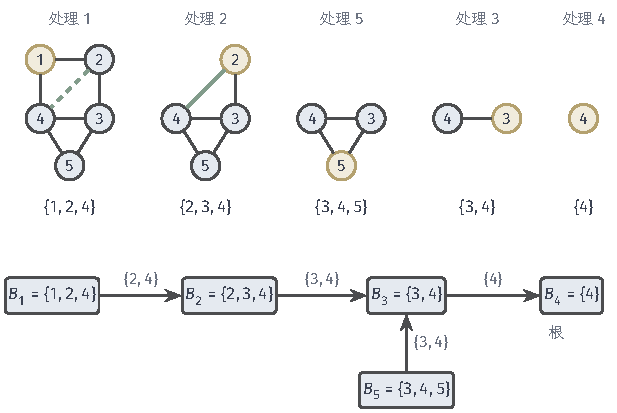
\includegraphics[width=104.369mm]{figures/01-basic-mathematics/04-graphs/tikz/c5-elimination-to-decomposition/figure.pdf}
  \caption{由消元次序$(1,2,5,3,4)$构造树分解。上行：每一轮的当前图，黄色为正在处理的顶点，绿色虚线为本轮补入的填充边，下一轮中它以绿色实线留在当前图里；图下标出记录的袋。下：按“连到最早被处理的后续邻居”连接父袋得到的袋树，箭头指向父袋，边旁标出接口。}
  \label{fig:graph-dp-elimination-to-decomposition}
\end{figure}

表中每个非根袋与父袋的接口恰好等于它的后续邻居集合。这不是巧合：父袋容纳$S_v$，而$v$本身比父袋的顶点都早被处理，不在父袋中，所以$B_v\cap B_{p(v)}=S_v$。第~\ref{sec:graph-dp-function-message-correspondence}小节会利用这一点把中间函数与袋之间的消息对应起来。

\subsection{从消元簇得到树分解}
\label{sec:graph-dp-clusters-to-decomposition}

下面的定理说明上述构造总是给出树分解，从而把消元过程中生成的依赖正式转成树分解，而不是另设一套独立的构建方法。

\begin{theorem}[消元次序产生树分解]
\label{thm:graph-dp-elimination-decomposition}
设$\mathcal G$是非空有限无向图，$R\subseteq V$，$\pi$是$V\setminus R$的消元次序。按算法~\ref{alg:graph-dp-order-to-decomposition}得到的袋树是$\mathcal G_R$的树分解，有保留集时根袋$B_R=R$；其宽度为$\pi$的诱导宽度与$|R|-1$中的较大者，无保留集时就是诱导宽度。特别地，$\mathcal G$的树宽不超过任何完整消元次序的诱导宽度。
\end{theorem}

\begin{proof}
先说明袋树是树。每个非根袋恰有一条通向父袋的边。父袋若为$B_{p(v)}$，则$p(v)$在次序中排在$v$之后，沿父边前进时次序位置严格增大；父袋若为$B_R$，则到达根袋。所以沿父边前进不会回到出发点，不形成环，每条父链都在有限步后到达一个根。各根之间再用树边连接，整体连通且无环。

顶点覆盖：待消去的$v$属于$B_v$，$R$中的顶点属于$B_R$。边覆盖：设$\{u,v\}$是$\mathcal G_R$的边。若两端都在$R$中，它被$B_R$覆盖。否则设$u$是两端中先被处理的待消去顶点；在处理$u$之前，图中只删去过已处理的顶点及其关联边，所以边$\{u,v\}$仍在，$v\in N^+_\pi(u)$，于是$B_u$同时含$u,v$。

运行交集：设$z\in B_v$且$z\neq v$，只需证明从$B_v$沿父链向上的每个袋都含$z$，直到到达$B_z$（$z$待消去时）或$B_R$（$z\in R$时）。这样含$z$的每个袋都与$B_z$或$B_R$由一条全部含$z$的路径相连，$T_z$连通。由$z\in N^+_\pi(v)=S_v$和上一小节的“父袋容纳剩余作用域”，父袋包含$S_v$，所以含$z$；若父袋是$B_{p(v)}$且$p(v)\neq z$，就对$p(v)$重复同样的论证。次序位置严格增大，最终到达$B_z$或$B_R$。

宽度：待消去顶点的袋大小为$|S_v|+1$，根袋大小为$|R|$，所以宽度如定理所述。最后，无保留集时树宽是全部树分解宽度的最小值，所以不超过诱导宽度。
\end{proof}

证明中的边覆盖论证同样适用于填充边，因此所得袋树也是填充图$\mathcal G^+_\pi$的树分解。

另一个直接推论是：每个局部函数的作用域$S_a$都整体落在某个袋中。取$S_a$中最先被处理的待消去变量$v$，$S_a$的其余变量在原始图中都与$v$相邻且排在$v$之后（或属于$R$），所以都在$S_v$中，$S_a\subseteq B_v$；若$S_a\subseteq R$，则$S_a\subseteq B_R$。第~\ref{sec:graph-dp-term-assignment}小节据此为局部项指定归属。

\paragraph{结构操作的代价}
设处理第$t$个顶点时它有$d_t$个当前邻居，补边要检查$\sum_t d_t(d_t-1)/2$对顶点，记录的袋共含$\sum_t(d_t+1)$个顶点。用支持常数时间查边和加边的邻接集合实现时，时间为
\[
O\Bigl(n+m+\sum_t d_t^2\Bigr),
\]
其中$m$是原始图的边数。这只是结构操作的开销；在袋上计算数值表时，开销随袋大小指数增长，第~\ref{sec:graph-dp-computation-cost}节另行计算。

% 第12章第3节：由树分解构建动态规划（包含局部作用域的袋、接口的分隔性质、从叶袋得到消元序）。

\section{由树分解构建动态规划}
\label{sec:graph-dp-from-decomposition}

上一节从消元次序出发得到树分解。本节反过来，从一个给定的树分解出发，直接规定局部子问题。需要证明的有两件事：每个局部项都能整体放进某个袋，这样它才有处可放；相邻两袋的接口确实把两侧的变量隔开，这样以接口为索引的摘要才足够。最后从叶袋向内处理变量，读出一个与分解相容的消元次序，说明树分解既能作为构建的输入，也能作为消元结果的显式表示。

\subsection{包含局部作用域的袋}
\label{sec:graph-dp-clique-containment}

计算时每个局部函数要整个放进一个袋，因为袋表需要同时索引它的全部变量。一个作用域$S_a$在原始图上是团：其中任意两个变量同在$\phi_a$中，因而相邻。但树分解的定义只要求每条边被某个袋覆盖，三个变量两两成边时，三条边似乎可能分别落在三个不同的袋中。下面先证明一个关于子树的一般事实，再由它推出这种情况不会发生。

把每个顶点$v$的出现位置$T_v$看成袋树中的一棵连通子树。若$u,v$相邻，边覆盖给出一个同时含$u,v$的袋，于是$T_u$与$T_v$相交。对一个团$C$，各$T_v$（$v\in C$）两两相交；要证明的是它们有一个公共节点。

\begin{lemma}[两两相交的子树有公共节点]
\label{lem:graph-dp-subtree-helly}
设$\mathcal T$是有限树，$T_1,\ldots,T_k$（$k\geq1$）是它的非空连通子树，并且两两相交。则存在节点同时属于全部$T_j$。
\end{lemma}

\begin{proof}
任取$\mathcal T$的一个节点作为根。与引理~\ref{lem:graph-dp-unique-internal}的证明相同，每个$T_j$有唯一一个离根最近的节点，记为$r_j$，并且$T_j$的每个节点都是$r_j$的后代（含$r_j$本身）。取$j^\ast$使$r_{j^\ast}$的深度在$r_1,\ldots,r_k$中最大，下面证明$r_{j^\ast}$属于每个$T_l$。

$l=j^\ast$时结论由定义成立。$l\neq j^\ast$时，$T_l\cap T_{j^\ast}$中有某个节点$x$；$x\in T_{j^\ast}$，因而$x$是$r_{j^\ast}$的后代。

考察$T_l$中从$x$到$r_l$的路径，它留在$T_l$中。若$r_l$不是$r_{j^\ast}$的后代，这条路径从$r_{j^\ast}$下方的子树走到外部，必须经过$r_{j^\ast}$，因为这棵子树与外部只通过$r_{j^\ast}$与其父节点之间的边相连；于是$r_{j^\ast}\in T_l$。若$r_l$是$r_{j^\ast}$的后代，则$r_l$的深度不小于$r_{j^\ast}$的深度；而按$j^\ast$的选取，$r_l$的深度又不大于$r_{j^\ast}$的深度，所以$r_l=r_{j^\ast}$，同样有$r_{j^\ast}\in T_l$。
\end{proof}

\begin{lemma}[团被某个袋容纳]
\label{lem:graph-dp-clique-in-bag}
设$(\mathcal T,\{B_t\}_{t\in T})$是$\mathcal G$的树分解，$C\subseteq V$是$\mathcal G$中的非空团，则存在节点$t\in T$使$C\subseteq B_t$。
\end{lemma}

\begin{proof}
由顶点覆盖与运行交集，每个$T_v$（$v\in C$）是非空连通子树。$C$中任意两个顶点$u,v$相邻，由边覆盖，$T_u\cap T_v\neq\varnothing$。由引理~\ref{lem:graph-dp-subtree-helly}，存在节点$t$属于全部$T_v$，即$C\subseteq B_t$。
\end{proof}

图~\ref{fig:graph-dp-clique-in-bag}画出了证明中的几棵子树：每个变量的出现位置向上延伸到自己的最高节点，最高节点最深的那个变量，它的最高节点被其余各子树“经过”，因而就是要找的袋。

\begin{figure}[!htb]
  \centering
  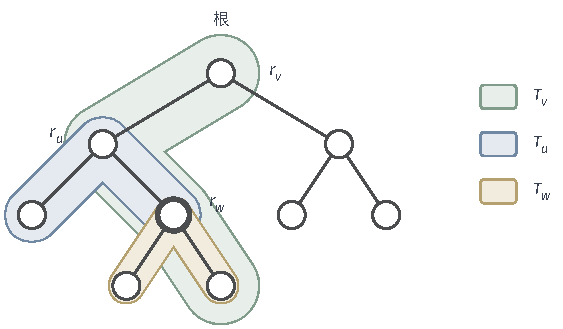
\includegraphics[width=102.648mm]{figures/01-basic-mathematics/04-graphs/tikz/c5-clique-in-bag/figure.pdf}
  \caption{团$\{u,v,w\}$被某个袋容纳的论证。袋树以顶部节点为根，三种颜色的区域分别是$T_u$、$T_v$、$T_w$，标签$r_u,r_v,r_w$标出各自离根最近的节点。$r_w$最深；$T_u$、$T_v$都要与$T_w$相交，而它们的最高节点不比$r_w$深，所以必须经过$r_w$。粗圈节点$r_w$的袋同时含$u,v,w$。}
  \label{fig:graph-dp-clique-in-bag}
\end{figure}

由引理~\ref{lem:graph-dp-clique-in-bag}，原始图的任一树分解中，每个局部函数的完整作用域都被某个袋整体容纳。因此在原始图上构造树分解就足够了，不需要额外记录高阶作用域；第~\ref{sec:graph-local-functions}节所说的“结构以原始图为依据、计算保留完整函数”在这里得到保证。

要找出容纳$S_a$的袋，只需在$T_v$（$v\in S_a$）中最小的一个里逐个检查袋是否包含$S_a$。同样，第~\ref{sec:graph-dp-query-structure}小节补成团的保留集$R$也一定被某个袋容纳。

\paragraph{树宽的下界}
引理~\ref{lem:graph-dp-subtree-helly}也给出第~\ref{sec:graph-tree-decomposition}小节几个例子的下界。一条边要求某个袋含两个顶点，所以含边的图宽度不能小于$1$；至少含一条边的树因而树宽恰为$1$。

四个顶点的环$1-2-3-4-1$没有宽度为$1$的树分解。给任一树分解选根，取环上的顶点$w$使$T_w$的最高节点最深。$w$在环上的两个邻居$u,v$各自与$w$相邻，于是$T_u$、$T_v$都与$T_w$相交；引理证明中的论证表明，$T_w$的最高节点同时属于$T_u$与$T_v$。这个袋含$u,v,w$三个顶点，所以宽度至少为$2$，四环的树宽恰为$2$。

这一论证对任何环都适用：含环的图树宽至少为$2$。因此树宽为$1$的图恰好是至少含一条边的森林。森林的各个分量分别按树的方法分解，再用任意的边把各分量的袋树连成一棵树；不同分量没有公共顶点，这些连接不影响运行交集。图~\ref{fig:graph-dp-ladder-decomposition}的梯子含环，又有宽度为$2$的分解，所以树宽恰为$2$；按同样的方式扫描，任意长的梯子树宽都是$2$。

四个顶点两两相邻的完全图恰好相反。整个顶点集是一个团，由引理~\ref{lem:graph-dp-clique-in-bag}，任何树分解都有一个袋装下全部四个顶点，宽度至少为$3$，所以树宽为$3$。同样，$n$个顶点的完全图树宽为$n-1$，树分解对它没有任何节省。

可见树宽衡量的是图与树的接近程度：一条边需要两个变量同时出现，一个环迫使某处至少三个变量同时出现，而一个大团迫使它的全部变量同时出现。

\subsection{接口的分隔性质}
\label{sec:graph-dp-interface-separation}

树上消息的正确性依赖于一件事：删去一条边后，两侧除了接收变量以外没有共同的变量。袋树上，这件事由运行交集保证。删去袋树边$\{s,t\}$后，袋树分成两部分；记$s$一侧全部袋中出现的变量为$V_{s|t}$，$t$一侧为$V_{t|s}$，接口为$B_s\cap B_t$。

若某个变量$v$在两侧都出现，从它在$s$侧的某个出现位置到$t$侧的某个出现位置，袋树路径必须经过边$\{s,t\}$；由运行交集，$B_s$与$B_t$都含$v$。所以
\begin{equation}
V_{s|t}\cap V_{t|s}\subseteq B_s\cap B_t,
\label{eq:graph-dp-interface-separation}
\end{equation}
即接口把两侧的变量隔开：固定接口取值后，两侧的其余变量互不重叠。

只有变量不重叠还不够，还要确认两侧没有被某个局部项直接连在一起，否则两侧的其余变量仍不能分别优化。下面的引理说明，每个局部项都整体落在某一侧。

\begin{lemma}[接口分隔两侧]
\label{lem:graph-dp-interface-separation}
设$(\mathcal T,\{B_t\}_{t\in T})$是原始图的树分解，$\{s,t\}$是袋树的边。则式~\eqref{eq:graph-dp-interface-separation}成立；并且对每个局部函数$\phi_a$，$S_a\subseteq V_{s|t}$或$S_a\subseteq V_{t|s}$。因此，任何局部项都不同时读取$V_{s|t}\setminus B_t$中的变量与$V_{t|s}\setminus B_s$中的变量。
\end{lemma}

\begin{proof}
式~\eqref{eq:graph-dp-interface-separation}已在上面证明。由引理~\ref{lem:graph-dp-clique-in-bag}，$S_a$被某个袋$B_x$容纳，$x$在$s$一侧或$t$一侧，于是$S_a\subseteq V_{s|t}$或$S_a\subseteq V_{t|s}$。若某个$\phi_a$同时读取$y\in V_{s|t}\setminus B_t$与$z\in V_{t|s}\setminus B_s$，不妨设$S_a\subseteq V_{s|t}$，则$z\in V_{s|t}\cap V_{t|s}\subseteq B_s$，与$z\notin B_s$矛盾；另一种情形同理。
\end{proof}

在选了根的袋树中，取$t=p(u)$。$u$下方各袋（含$u$本身）中出现而不在接口$S_u$中的变量，由式~\eqref{eq:graph-dp-interface-separation}不会出现在其余袋中，它们正是$u$下方各节点的内部变量之并。引理~\ref{lem:graph-dp-interface-separation}说明，固定$\bm x_{S_u}$后，这些变量与其余变量之间没有遗漏的直接耦合，所以$u$下方可以单独摘要成一张以$\bm x_{S_u}$为索引的表。这正是第~\ref{sec:graph-dp-construction-goal}小节的第二项要求；第~\ref{sec:graph-dp-min-cost-correctness}小节用它证明数值递推的正确性。

\subsection{从叶袋得到消元序}
\label{sec:graph-dp-decomposition-to-order}

给定一个宽度为$w$的树分解，可以反过来读出一个诱导宽度不超过$w$的消元次序。思路是从叶袋开始：叶袋中不在父袋里的变量只出现在这个叶袋中，消去它们时，它们的邻居都在叶袋里，产生的填充边也都落在叶袋里。

\paragraph{算法}
输入是图$\mathcal G$的一个树分解，选定一个根；输出是全部顶点的一个消元次序。维护当前图（初值为$\mathcal G$）、当前袋树（初值为输入分解）和已输出的次序（初值为空）。当前袋树不只一个节点时，反复处理一个非根叶节点$\ell$，记其父节点为$p$：
\begin{itemize}
  \item 若$B_\ell\subseteq B_p$，直接从袋树中删去$\ell$；
  \item 否则按任意次序依次消去$B_\ell\setminus B_p$中的变量：把每个变量追加到次序末尾，在当前图中把它的邻居补成团并删去它，同时把它从$B_\ell$中删去；此时$B_\ell\subseteq B_p$，再删去$\ell$。
\end{itemize}
最后只剩根袋，按任意次序消去其中剩余的变量。

\begin{algorithm}[由树分解读出消元次序]
\label{alg:graph-dp-decomposition-to-order}
输入：有限无向图$\mathcal G$的树分解，以及选定的根。输出：$\mathcal G$的一个消元次序。
\begin{enumerate}
  \item 令当前图为$\mathcal G$的副本，当前袋树为输入的分解，次序为空。
  \item 若当前袋树只剩根，转第4步。否则取一个非根叶节点$\ell$及其父节点$p$。
  \item 依次消去$B_\ell\setminus B_p$中的变量（追加到次序、补团、从当前图和$B_\ell$中删去），然后删去节点$\ell$，回到第2步。
  \item 按任意次序消去根袋中剩余的变量，输出次序。
\end{enumerate}
\end{algorithm}

\paragraph{正确性}
算法维持一个不变量：当前袋树（各袋只保留尚未消去的变量）是当前图的树分解。开始时它就是输入分解。

设叶节点$\ell$中有变量$v\notin B_p$。由运行交集，$T_v$连通，而$\ell$在袋树中只与$p$相邻、$p\notin T_v$，所以$T_v=\{\ell\}$：$v$只出现在$B_\ell$中。由边覆盖，$v$在当前图中的每条边都被某个含$v$的袋覆盖，只能是$B_\ell$，所以$v$的当前邻居全在$B_\ell$中，个数至多$|B_\ell|-1\leq w$。消去$v$补入的填充边两端都在$B_\ell$中，被$B_\ell$覆盖；从$B_\ell$中删去$v$后，三个条件对新的当前图仍然成立。

$B_\ell\subseteq B_p$时删去$\ell$也保持不变量：$\ell$覆盖的顶点和边都被$B_p$覆盖；含某个变量的节点集合去掉一个叶节点后仍然连通。最后剩下根袋时，当前图的全部顶点都在根袋中，每个顶点的当前邻居至多$|B_r|-1\leq w$个。

所以每个顶点被消去时，剩余邻居数都不超过$w$，得到的消元次序诱导宽度不超过分解的宽度。

\paragraph{执行过程}
以图~\ref{fig:graph-dp-ladder-decomposition}的梯子为例，以$\{3,5,6\}$为根，逐步处理叶袋：
\begin{itemize}
  \item 叶袋$\{1,2,4\}$的父袋是$\{2,4,5\}$，消去$1$：它的当前邻居为$\{2,4\}$，补入$\{2,4\}$；剩余的$\{2,4\}$包含于父袋，删去该叶。
  \item 接着$\{2,4,5\}$成为叶，消去$4$：当前邻居为$\{2,5\}$，已相邻。
  \item 再处理$\{2,3,5\}$，消去$2$：当前邻居为$\{3,5\}$，补入$\{3,5\}$。
  \item 最后在根袋中依次消去$3,5,6$。
\end{itemize}

得到的次序为$(1,4,2,3,5,6)$，各步剩余邻居数依次为$2,2,2,2,1,0$，诱导宽度为$2$，等于分解的宽度。每一步补入的填充边都落在当时的叶袋里，正如正确性论证所说。

% 第12章第4节：两种构建的等价关系（中间函数与接口消息的对应、树宽与最小诱导宽度、四环上的双向构建）。

\section{两种构建的等价关系}
\label{sec:graph-dp-construction-equivalence}

前两节分别从消元次序和树分解出发，构建出同一类结构。本节把两种表示逐项对照：消元簇对应袋，剩余作用域对应接口，中间函数对应向父袋传递的消息。比较规模时，要区分某一个构建的宽度与全部构建中的最优值；后者在两种表示下相等。最后在四环上把双向转换逐步做一遍。

\subsection{中间函数与接口消息的对应}
\label{sec:graph-dp-function-message-correspondence}

在算法~\ref{alg:graph-dp-order-to-decomposition}得到的袋树中，取消元森林的根为根。每个非根袋$B_i=\{v_i\}\cup S_i$与父袋的接口恰为$S_i$：第~\ref{sec:graph-dp-order-to-decomposition}小节已说明父袋包含$S_i$；另一方面，父袋若是$B_j=\{v_j\}\cup S_j$，其中的变量在处理$v_j$时都还在当前图中，而$v_i$此前已被删去，所以$v_i\notin B_j$，父袋若是根袋$B_R$，也因$v_i\notin R$而不含$v_i$。所以$B_i$的内部变量只有$v_i$一个，这与引理~\ref{lem:graph-dp-unique-internal}一致：$v_i$所在的最高节点就是$B_i$。

于是两种表示中的对象逐项对应：
\begin{itemize}
  \item 第$i$步的消元簇$B_i$对应袋树的一个节点；
  \item 中间函数$\psi_i$的作用域$S_i$对应该节点与父节点的接口；
  \item 消去$v_i$对应汇总该节点的内部变量；
  \item “$\psi_i$在消去$S_i$中最早的变量时被使用”对应“消息从子节点发往父节点”。
\end{itemize}
第~\ref{sec:graph-dp-elimination-message-correspondence}小节在相同的局部项归属下证明，按消元次序算出的$\psi_i$与沿袋树算出的消息逐项相等。

反过来，算法~\ref{alg:graph-dp-decomposition-to-order}从树分解读出消元次序时，处理叶袋$\ell$就是一次消息传递：消去$B_\ell\setminus B_p$中的变量，留下以$B_\ell\cap B_p$为作用域的结果交给父袋。一个袋可以有多个内部变量，相当于把连续的几步消元合并在一个计算单元里完成。

对应关系不要求逐表相同。把相邻的袋合并、把一个局部项从一个容纳它的袋移到另一个，都会改变中间表；只要结果仍是合法的树分解、每个局部项的作用域被所归的袋容纳、每项恰好归入一处，最终的最小成本、条件最小成本表、计数和加权总和都不变。这一点在第~\ref{chap:general-graph-dp-computation}章随各任务的正确性一起证明。

\paragraph{两种表示的组织差别}
两种做法的差别在于组织方式。变量消元边走边决定新函数交给谁，结构与数值交织在一起；树分解先把结构确定下来并核验，同一个分解可以用于作用域相同而数值不同的多组局部函数，也便于在不同的根下重复使用，例如第~\ref{sec:graph-dp-tree-two-pass}小节那样再发一遍反向消息，得到每个袋上的表。

\subsection{树宽与最小诱导宽度}
\label{sec:graph-dp-treewidth-induced-width}

定理~\ref{thm:graph-dp-elimination-decomposition}给出一个方向：每个消元次序都产生宽度等于其诱导宽度的树分解。第~\ref{sec:graph-dp-decomposition-to-order}小节给出另一个方向：每个宽度为$w$的树分解都读出诱导宽度不超过$w$的消元次序。两个方向合起来，得到下面的等式。

\begin{theorem}[树宽等于最小诱导宽度]
\label{thm:graph-dp-treewidth-induced-width}
设$\mathcal G$是非空有限无向图。则
\[
\operatorname{tw}(\mathcal G)=\min_{\pi}\ \max_{v}\ |N^+_\pi(v)|,
\]
其中$\pi$取遍全部顶点的消元次序，$N^+_\pi(v)$是按$\pi$消元时$v$的剩余邻居集合。
\end{theorem}

\begin{proof}
记右端为$w^\ast$，它是有限个次序上的最小值，因而可以达到。由定理~\ref{thm:graph-dp-elimination-decomposition}，诱导宽度为$w^\ast$的次序给出宽度为$w^\ast$的树分解，所以$\operatorname{tw}(\mathcal G)\leq w^\ast$。反过来，取宽度为$\operatorname{tw}(\mathcal G)$的树分解，由算法~\ref{alg:graph-dp-decomposition-to-order}及其正确性论证，得到诱导宽度不超过$\operatorname{tw}(\mathcal G)$的次序，所以$w^\ast\leq\operatorname{tw}(\mathcal G)$。
\end{proof}

这个等式说的是两种表示的最优值相等，不是两种对象一一对应。同一个树分解按不同的根、不同的叶袋处理次序可以读出许多消元次序；不同的消元次序也可能给出合并后相同的袋树。等式的用途是：寻找好的结构时，可以在消元次序上搜索，也可以在树分解上搜索，二者的最优规模相同。对某一个具体次序或分解，它的宽度只是树宽的上界。

\subsection{四环上的双向构建}
\label{sec:graph-dp-four-cycle-construction}

现在在四环算例上把两个方向逐步做一遍。原始图是环$1-2-3-4-1$。

\paragraph{由消元次序到袋树}
按次序$(1,2,3,4)$执行算法~\ref{alg:graph-dp-order-to-decomposition}，表~\ref{tab:graph-dp-four-cycle-construction}列出每一轮的状态。消去$1$时补入填充边$\{2,4\}$；消去$2$时当前邻居为$\{3,4\}$，已经相邻；之后不再补边。

\begin{table}[!htb]
  \centering
  \caption{四环上按次序$(1,2,3,4)$构建袋树。“当前邻居”从上一轮更新后的图读取；父袋按“后续邻居中次序最早者”确定，最后一列是与父袋的接口，它恰好等于当前邻居集合。}
  \label{tab:graph-dp-four-cycle-construction}
  \small
  \begin{tabular}{@{}ccccccc@{}}
    \toprule
    轮 & 消去 & 当前邻居$S_i$ & 填充边 & 消元簇$B_i$ & 父袋 & 接口\\
    \midrule
    $1$ & $1$ & $\{2,4\}$ & $\{2,4\}$ & $\{1,2,4\}$ & $B_2$ & $\{2,4\}$\\
    $2$ & $2$ & $\{3,4\}$ & 无 & $\{2,3,4\}$ & $B_3$ & $\{3,4\}$\\
    $3$ & $3$ & $\{4\}$ & 无 & $\{3,4\}$ & $B_4$ & $\{4\}$\\
    $4$ & $4$ & $\varnothing$ & 无 & $\{4\}$ & 根 & —\\
    \bottomrule
  \end{tabular}
\end{table}

得到的袋树是一条路径$\{1,2,4\}-\{2,3,4\}-\{3,4\}-\{4\}$，宽度为$2$。后两个袋包含于$\{2,3,4\}$，把它们并入后只剩$\{1,2,4\}-\{2,3,4\}$，接口为$\{2,4\}$，这就是第~\ref{sec:graph-dp-four-cycle}小节计算时使用的两个子问题。可以逐条核对定义：四条环边$\{1,2\},\{1,4\}$在第一个袋，$\{2,3\},\{3,4\}$在第二个袋；含$2$或$4$的袋相邻，含$1$或$3$的袋只有一个。

\paragraph{由袋树到消元次序}
反过来，从分解$\{1,2,4\}-\{2,3,4\}$出发执行算法~\ref{alg:graph-dp-decomposition-to-order}。以$\{2,3,4\}$为根时，叶袋$\{1,2,4\}$中不在父袋里的变量是$1$，先消去$1$，再在根袋中按$2,3,4$消去，读回次序$(1,2,3,4)$。

以$\{1,2,4\}$为根时，叶袋变成$\{2,3,4\}$，不在父袋里的变量是$3$。消去$3$时它在环上的当前邻居是$\{2,4\}$，补入$\{2,4\}$，这条填充边落在叶袋里；随后在根袋中按$1,2,4$消去，得到次序$(3,1,2,4)$，各步剩余邻居数为$2,2,1,0$。两个次序补入的是同一条填充边，诱导宽度都是$2$。

\paragraph{两种表示的对照}
两种表示中，最多同时处理的变量都是三个：消元簇$\{1,2,4\}$、$\{2,3,4\}$就是两个袋。由定理~\ref{thm:graph-dp-treewidth-induced-width}和第~\ref{sec:graph-dp-clique-containment}小节的下界，四环的树宽为$2$，所以四环上任何消元次序的诱导宽度都至少是$2$，这里的两个次序已经最优。

另一种同样宽度的分解是$\{1,2,3\}-\{1,3,4\}$，接口为$\{1,3\}$，它对应先消去$2$或$4$、补入$\{1,3\}$的次序。第~\ref{sec:graph-dp-query-structure}小节的保留集$R=\{1,3\}$要求的正是这种结构：在补边$\{1,3\}$后的图上只消去$V\setminus R$，按次序$(2,4)$执行算法~\ref{alg:graph-dp-order-to-decomposition}，消去$2$时$S_2=\{1,3\}\subseteq R$，消去$4$时$S_4=\{1,3\}\subseteq R$，两个消元簇$\{1,2,3\}$与$\{1,3,4\}$都连到根袋$B_R=\{1,3\}$。第~\ref{sec:graph-dp-retained-check}小节在这个结构上计算条件最小成本表。

% 第12章第5节：构造策略（消元次序的选择、弦图与完美消元序、完美消元序的构造与核验、团树的构造、构建结果的检验）。

\section{构造策略}
\label{sec:graph-tree-decomposition-construction}

前几节说明了消元次序与树分解怎样互相转换，但没有说明怎样得到规模小的结构。本节在已经建立的等价关系上讨论实际构造：用局部规则选择消元次序；在弦图上利用不需补边的完美消元序；把弦图的极大团借第~\ref{chap:minimum-spanning-tree}章的最大权生成树连成团树；最后逐项检验构建结果。本节的算法只做结构操作，输出袋和袋之间的连接，不计算数值表；输出中实际的袋大小是第~\ref{sec:graph-dp-computation-cost}节代价分析的输入。

\subsection{消元次序的选择}
\label{sec:graph-dp-order-heuristics}
\label{sec:graph-dp-elimination-orders}

\subsubsection{次序对消元簇的影响}

由定理~\ref{thm:graph-dp-elimination-decomposition}，任何消元次序都给出合法的结构，但不同次序产生的消元簇可以相差很多。在三元作用域例子上比较两种次序：$(1,4,2,3)$与先消$x_2$的$(2,1,3,4)$。前者每一步被消去的顶点的邻居都已两两相邻，不产生填充边，消元簇依次为$\{1,2,3\},\{2,3,4\},\{2,3\},\{3\}$。后者第一步要处理$\{1,2,3,4\}$并补入$\{1,4\}$，此后的消元簇为$\{1,3,4\},\{3,4\},\{4\}$。表~\ref{tab:graph-dp-elimination-orders}列出了两种次序每一步的作用域和规模，图~\ref{fig:graph-dp-elimination-orders}画出了对应的图变化。

\begin{table}[!htb]
  \centering
  \caption{三元作用域例子上两种消元次序的逐步规模。“枚举”指计算新函数时要比较的候选组合数，即消元簇上的配置数；“输出”指新函数表的项数，回溯表的项数与之相同。}
  \label{tab:graph-dp-elimination-orders}
  \begin{tabular}{cccccccc}
    \toprule
    \multicolumn{4}{c}{次序$(1,4,2,3)$} & \multicolumn{4}{c}{次序$(2,1,3,4)$}\\
    \cmidrule(lr){1-4}\cmidrule(lr){5-8}
    消去 & 新作用域 & 枚举 & 输出 & 消去 & 新作用域 & 枚举 & 输出\\
    \midrule
    $x_1$ & $\{2,3\}$ & $8$ & $4$ & $x_2$ & $\{1,3,4\}$ & $16$ & $8$\\
    $x_4$ & $\{2,3\}$ & $8$ & $4$ & $x_1$ & $\{3,4\}$ & $8$ & $4$\\
    $x_2$ & $\{3\}$ & $4$ & $2$ & $x_3$ & $\{4\}$ & $4$ & $2$\\
    $x_3$ & $\varnothing$ & $2$ & $1$ & $x_4$ & $\varnothing$ & $2$ & $1$\\
    \midrule
    合计 & & $22$ & $11$ & 合计 & & $30$ & $15$\\
    \bottomrule
  \end{tabular}
\end{table}

\begin{figure}[!htb]
  \centering
  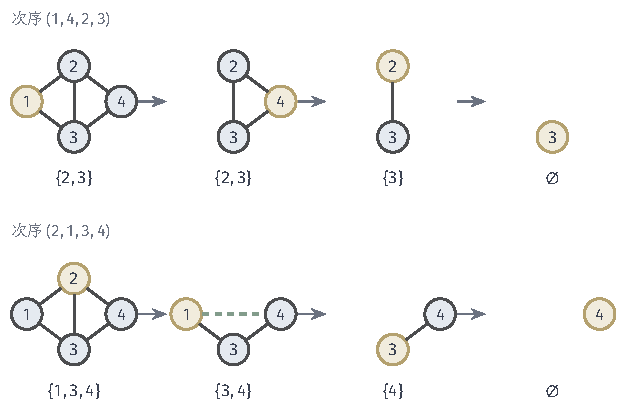
\includegraphics[width=105.004mm]{figures/01-basic-mathematics/04-graphs/tikz/c5-elimination-orders/figure.pdf}
  \caption{两种消元次序下原始图的变化。上行按$(1,4,2,3)$消元，每一步被消去的黄色顶点的邻居都已两两相邻，不产生填充边，新函数至多读取两个变量。下行按$(2,1,3,4)$消元，消去$2$时要补入填充边$\{1,4\}$（第二个图中的绿色虚线），新函数读取三个变量。每个图下方标出消去黄色顶点后新函数的作用域。}
  \label{fig:graph-dp-elimination-orders}
\end{figure}

第一种次序的最大中间表只有$4$项，第二种有$8$项。在这个小例子里差别不大；但若每个变量有$q$个状态，读取$r$个变量的表就有$q^r$项，多读取一个变量意味着表扩大$q$倍。

次序选得不好时，即使在树上也会产生大表：在第~\ref{sec:graph-dp-tree-messages}小节的分叉树上先消去中心$3$，它的邻居$1,2,4$两两补边，新函数要读取三个变量；而按后序消元时不产生任何填充边。两种次序算出的最小值相同（第~\ref{sec:graph-dp-min-cost-correctness}小节），差别只在中间表的规模。

\subsubsection{贪心规则}

定理~\ref{thm:graph-dp-treewidth-induced-width}把找好的树分解归结为找诱导宽度小的消元次序。在一般图上找诱导宽度最小的次序是困难的组合问题，实践中常用局部规则逐轮挑选顶点，得到一个可用但不保证最优的次序。

消去一个顶点，就是把它的全部当前邻居拉进同一个袋，并让它们两两相邻。代价因此体现在两处：它的当前邻居越多，这一步的袋越大；邻居之间缺的边越多，要补的填充边越多，剩下的图越稠密，以后的袋也可能越大。据此有两条常见规则：\term{最小度启发式}（min-degree），选当前邻居最少的顶点；\term{最小填充启发式}（min-fill），选消去时需要补边最少的顶点，即当前邻域中缺少的边数最少者。两条规则都只看当前这一步。

\paragraph{算法实现}

原图和评分规则在运行中不变。算法维护三项状态：
\begin{itemize}
  \item 当前图：初值为原图的副本；
  \item 已输出的次序：初值为空；
  \item 各轮的袋和填充边：初值为空。
\end{itemize}
每一轮依次做三件事：
\begin{itemize}
  \item 评分：在当前图上为每个剩余顶点计算评分，即当前度数或当前缺边数；
  \item 选择：取评分最小者，评分相同时取编号最小者，记为$v$；
  \item 消去：记录袋$\{v\}\cup N(v)$，其中$N(v)$是$v$的当前邻居，把$N(v)$补成团并记录填充边，删去$v$，把$v$追加到次序末尾。
\end{itemize}
当前图为空时停止。

\begin{algorithm}[贪心选择消元次序]
\label{alg:graph-dp-greedy-order}
输入：非空有限无向图和一条评分规则（当前度数或当前缺边数）。输出：消元次序、各轮的袋和填充边。
\begin{enumerate}
  \item 对当前图中的每个顶点按规则计算评分，取评分最小者，评分相同时取编号最小者，记为$v$。
  \item 记录袋$\{v\}\cup N(v)$，把$N(v)$补成团，删去$v$，并把$v$追加到次序末尾。
  \item 若图非空，回到第1步，并在更新后的图上重新计算评分。
\end{enumerate}
\end{algorithm}

评分必须在每轮更新后的图上重算。若只按初始度数排一次序，或用原图的缺边数代替当前缺边数，得到的就不是这两条规则，因为补边会改变其他顶点的度数和邻域。

\paragraph{执行过程}
图~\ref{fig:graph-dp-min-degree-min-fill}的图有六个顶点和边$\{1,3\},\allowbreak\{1,4\},\allowbreak\{1,5\},\allowbreak\{1,6\},\allowbreak\{2,3\},\allowbreak\{2,4\},\allowbreak\{2,6\},\allowbreak\{3,5\},\allowbreak\{4,5\},\allowbreak\{5,6\}$。初始度数依次为$4,3,3,3,4,3$；缺边数依次为$3,3,2,2,3,2$，例如顶点$2$的邻居$3,4,6$两两不相邻，缺$3$条边，而顶点$3$的邻居$1,2,5$中只缺$\{1,2\}$与$\{2,5\}$。表~\ref{tab:graph-dp-greedy-order-trace}并列两条规则的各轮结果。

最小度规则的执行如下：
\begin{itemize}
  \item 第$1$轮：度数为$3$的有$2,3,4,6$，按编号选$2$，袋为$\{2,3,4,6\}$，补入$\{3,4\},\allowbreak\{3,6\},\allowbreak\{4,6\}$。
  \item 第$2$轮：剩下的五个顶点因此两两相邻，度数都是$4$，按编号选$1$，袋为$\{1,3,4,5,6\}$，宽度升到$4$。
  \item 第$3$至$6$轮：剩余图始终是完全图，依次选$3,4,5,6$，不再补边。
\end{itemize}
最小填充规则的执行如下：
\begin{itemize}
  \item 第$1$轮：缺边数为$2$的有$3,4,6$，按编号选$3$，袋为$\{1,2,3,5\}$，补入$\{1,2\}$与$\{2,5\}$。
  \item 第$2$轮：$4$的邻居$1,2,5$已两两相邻，缺边数为$0$；$6$的缺边数也是$0$，按编号选$4$，袋为$\{1,2,4,5\}$。
  \item 第$3$至$6$轮：剩下的四个顶点两两相邻，依次选$1,2,5,6$，不再补边。
\end{itemize}
最大袋含$4$个顶点，宽度为$3$，比最小度规则少$1$。

\begin{table}[!htb]
  \centering
  \caption{两条贪心规则在图~\ref{fig:graph-dp-min-degree-min-fill}的六顶点图上的各轮结果。“选中”列括号内是该顶点当轮的评分（最小度规则为当前度数，最小填充规则为当前缺边数），“补边”列是该轮补入的填充边条数。}
  \label{tab:graph-dp-greedy-order-trace}
  \small
  \begin{tabular}{@{}ccccccc@{}}
    \toprule
    & \multicolumn{3}{c}{最小度} & \multicolumn{3}{c}{最小填充}\\
    \cmidrule(lr){2-4}\cmidrule(lr){5-7}
    轮 & 选中 & 袋 & 补边 & 选中 & 袋 & 补边\\
    \midrule
    $1$ & $2$（$3$） & $\{2,3,4,6\}$ & $3$ & $3$（$2$） & $\{1,2,3,5\}$ & $2$\\
    $2$ & $1$（$4$） & $\{1,3,4,5,6\}$ & $0$ & $4$（$0$） & $\{1,2,4,5\}$ & $0$\\
    $3$ & $3$（$3$） & $\{3,4,5,6\}$ & $0$ & $1$（$0$） & $\{1,2,5,6\}$ & $0$\\
    $4$ & $4$（$2$） & $\{4,5,6\}$ & $0$ & $2$（$0$） & $\{2,5,6\}$ & $0$\\
    $5$ & $5$（$1$） & $\{5,6\}$ & $0$ & $5$（$0$） & $\{5,6\}$ & $0$\\
    $6$ & $6$（$0$） & $\{6\}$ & $0$ & $6$（$0$） & $\{6\}$ & $0$\\
    \midrule
    宽度 & \multicolumn{3}{c}{$4$} & \multicolumn{3}{c}{$3$}\\
    \bottomrule
  \end{tabular}
\end{table}

\begin{figure}[!htb]
  \centering
  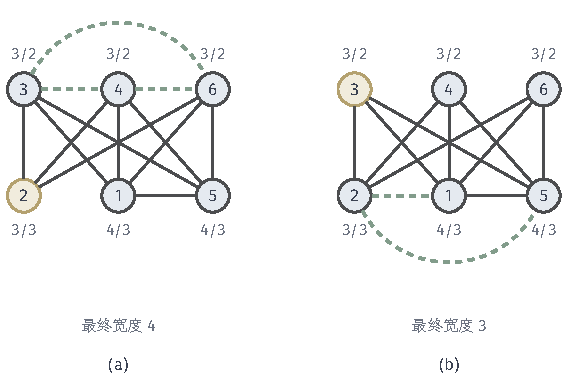
\includegraphics[width=96.778mm]{figures/01-basic-mathematics/04-graphs/tikz/c5-min-degree-min-fill/figure.pdf}
  \caption{最小度规则与最小填充规则的第一步。每个顶点旁的“$d/f$”是当前度数与当前缺边数。左：最小度规则在度数为$3$的顶点中按编号选$2$（黄色），要补三条绿色虚线，最终宽度为$4$。右：最小填充规则选缺边最少的$3$（黄色），只补两条边，最终宽度为$3$。}
  \label{fig:graph-dp-min-degree-min-fill}
\end{figure}

\subsubsection{贪心规则的分析}

\paragraph{启发式的局限}
两种规则都只看一步：度数小不代表补边少，补边少也不保证以后的袋小。上例中最小度规则受平局规则影响，第一步补的三条边把剩余图变成了完全图，得到的宽度比最小填充多$1$。穷举全部$720$个消元次序可以核对，这个图上任何次序的诱导宽度都不小于$3$，所以最小填充在这里恰好达到了最好的次序。换一个图，最小填充同样可能不是最优。因此报告结果时应分开写出构造的宽度、填充边数和结构操作次数，并把宽度理解为树宽的上界，而不是树宽本身。

宽度按变量个数计，而表的项数按状态数之积计。各变量状态数不同时，诱导宽度相同的两个次序，其最大消元簇的配置数可以相差很多；这时可以把评分换成消元簇上的状态数之积，或者构造后直接比较各簇的实际配置数。第~\ref{sec:graph-dp-table-size}小节按实际乘积比较候选结构。

\paragraph{复杂度}
直接实现时每轮要为全部剩余顶点重算评分。最小度规则的评分只需读出度数；最小填充规则要检查每个顶点的每对邻居是否相邻，一轮的检查量可达$\sum_v|N(v)|^2$。用缓存时只重算受影响的顶点：加入边$\{a,b\}$只改变$a$、$b$及其公共邻居的评分，删去$v$只改变$v$的邻居的评分。

\subsection{弦图与完美消元序}
\label{sec:graph-dp-chordal}

填充边会使袋变大，最理想的情形是全程不需要补边。处理顶点$v$时不需要补边，当且仅当$v$的当前邻居已经两两相邻。当前邻居构成团的顶点称为\term{单纯顶点}（simplicial vertex）；没有邻居或只有一个邻居的顶点也算单纯顶点。若一个消元次序使每个顶点在被处理时都是当前图中的单纯顶点，就称它为\term{完美消元序}（perfect elimination ordering）。沿完美消元序消元不产生任何填充边，当前图始终是原图在剩余顶点上的诱导子图。

\paragraph{弦图}
不是每个图都有完美消元序。四个顶点的环$1-2-3-4-1$中，每个顶点的两个邻居都不相邻：$1$与$3$的邻居都是$\{2,4\}$，缺边$\{2,4\}$；$2$与$4$的邻居都是$\{1,3\}$，缺边$\{1,3\}$。所以第一步就找不到单纯顶点。补入边$\{1,3\}$后，顶点$2$的邻居$\{1,3\}$相邻，可以先消去；剩下的三角形$1,3,4$中每个顶点都单纯，于是$(2,1,3,4)$是完美消元序。图~\ref{fig:graph-dp-chordal-four-cycle}画出了这一对比。

\begin{figure}[!htb]
  \centering
  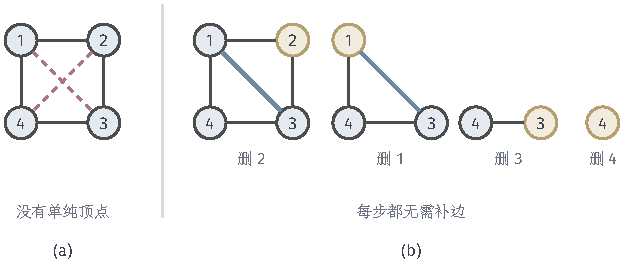
\includegraphics[width=106.306mm]{figures/01-basic-mathematics/04-graphs/tikz/c5-chordal-four-cycle/figure.pdf}
  \caption{无弦四环与补弦后的图。左：四环中每个顶点的两个邻居都不相邻（红色虚线为所缺的边），没有单纯顶点。右：补入弦$\{1,3\}$（蓝色）后，按$(2,1,3,4)$逐个删除，每一步被删除的黄色顶点的剩余邻居都已相邻，全程无填充。}
  \label{fig:graph-dp-chordal-four-cycle}
\end{figure}

四环的问题出在“长度至少为四而没有捷径的环”。消去这种环上的任何一个顶点，它在环上的两个邻居都不相邻，必须补一条边把它们直接连起来；三角形则没有这个问题，因为两个邻居本来就相邻。在长度至少为$4$的环上，连接两个在环上不相邻的顶点的边称为该环的\term{弦}（chord），也就是一条捷径。每个长度至少为$4$的环都有弦的有限无向图称为\term{弦图}（chordal graph）。

树没有环，是弦图；补入$\{1,3\}$后的四环是弦图；无弦四环不是。给一般图补边使之成为弦图称为\term{弦化}（chordal completion）。

\begin{theorem}[弦图与完美消元序]
\label{thm:graph-dp-chordal-peo}
有限无向图是弦图，当且仅当它有完美消元序。
\end{theorem}

\begin{proof}
先证有完美消元序的图是弦图。设图中有长度至少为$4$且无弦的环，考察环上最先被处理的顶点$v$。$v$在环上的两个邻居$u,w$此时都还在图中，并且与$v$相邻。$v$是单纯顶点，所以$u,w$相邻；而沿完美消元序处理时从不补边，$\{u,w\}$必是原图的边。环长至少为$4$，$u,w$在环上不相邻，于是$\{u,w\}$是这个环的弦，矛盾。

反方向的论证路线如下。第一步是一个引理：每个非空有限弦图都有单纯顶点，若它不是完全图，还有两个不相邻的单纯顶点。这一步需要分析极小分隔集，证明极小分隔集在弦图中都是团，本书不展开。第二步，弦图的诱导子图仍是弦图，因为诱导子图中的无弦环在原图中也无弦。于是可以反复删去一个单纯顶点，余下的图仍是弦图、仍有单纯顶点，直到删完，删除的次序就是完美消元序。
\end{proof}

\paragraph{填充图与弦化}
一般图经一次完整消元得到的填充图$\mathcal G^+_\pi$（第~\ref{sec:graph-dp-fill-in}小节）总是弦图，并且$\pi$就是它的完美消元序。要验证这一点，只需说明在$\mathcal G^+_\pi$中，$v$排在它之后的邻居恰是消元时的剩余邻居$N^+_\pi(v)$：$\mathcal G^+_\pi$中连接$v$与某个较晚顶点$w$的边，若是原始边，处理$v$时仍在；若是填充边，它在处理某个更早的顶点时补入，那时$v$还没有被删去，所以处理$v$时这条边也在。于是这些后续邻居在处理$v$时已被补成团，$v$在$\mathcal G^+_\pi$中按$\pi$处理时总是单纯顶点。由定理~\ref{thm:graph-dp-chordal-peo}，$\mathcal G^+_\pi$是弦图，第~\ref{sec:graph-dp-order-to-decomposition}小节的构造实际上隐含了一次弦化。

反过来，设$\mathcal H$是包含$\mathcal G$的弦图（顶点相同、边更多），$\sigma$是$\mathcal H$的完美消元序。按$\sigma$对$\mathcal G$消元，对步数归纳可知当前图始终是$\mathcal H$在剩余顶点上的诱导子图的子图：处理$v$时，它的当前邻居包含在$\mathcal H$中$v$的后续邻居里，后者在$\mathcal H$中成团，所以补入的填充边都是$\mathcal H$的边。因此$\mathcal G^+_\sigma\subseteq\mathcal H$，每个消元簇都含于$\mathcal H$的某个团，诱导宽度不超过$\mathcal H$的最大团大小减一。

这样，消元次序与弦化相互对应：选一个次序就选定了一个弦化，选一个弦化及其完美消元序也就得到一个宽度不更大的次序。四环算例按$(1,2,3,4)$消元，填充图是环加上弦$\{2,4\}$，$(1,2,3,4)$正是它的完美消元序；按$(2,1,3,4)$消元则对应图~\ref{fig:graph-dp-chordal-four-cycle}中补弦$\{1,3\}$的弦化。

\subsection{完美消元序的构造与核验}
\label{sec:graph-dp-peo-construction}

\subsubsection{问题与思路}

定理~\ref{thm:graph-dp-chordal-peo}只说明弦图有完美消元序，没有给出求法。输入是一个有限无向图，输出是它的一个完美消元序，或者“不是弦图”的报告及证据。定理证明的反方向已经提示了做法：反复找一个单纯顶点删去。弦图的每个诱导子图仍有单纯顶点，所以对弦图这一过程不会卡住；非弦图没有完美消元序，过程必然在某一轮找不到单纯顶点，这时剩下的图本身就是证据。

\subsubsection{算法实现}

输入图在运行中不变。算法维护两项状态：
\begin{itemize}
  \item 当前图：初值为输入图的副本；
  \item 已输出的次序：初值为空。
\end{itemize}
每一轮依次做两件事：
\begin{itemize}
  \item 检查：按编号逐个检查当前图中的顶点，枚举它的每对邻居看是否相邻，遇到第一个单纯顶点就停下；
  \item 删除：把找到的单纯顶点从当前图中删去，追加到次序末尾。
\end{itemize}
当前图为空时停止，输出的次序就是完美消元序。若非空的当前图中找不到单纯顶点，就停止并报告输入不是弦图，返回这个当前图作为证据，而不暗中补边。

\begin{algorithm}[逐次删除单纯顶点]
\label{alg:graph-dp-peo-construction}
输入：有限无向图。输出：完美消元序，或“不是弦图”的报告及当前图。
\begin{enumerate}
  \item 令当前图为输入图的副本，次序为空。
  \item 若当前图为空，输出次序并停止。
  \item 按编号检查当前图的顶点，找出第一个邻居两两相邻的顶点$v$；若不存在，报告输入不是弦图，返回当前图并停止。
  \item 从当前图中删去$v$，把$v$追加到次序末尾，回到第2步。
\end{enumerate}
\end{algorithm}

\paragraph{执行过程}
在补弦后的四环上（边$\{1,2\},\allowbreak\{2,3\},\allowbreak\{3,4\},\allowbreak\{1,4\},\allowbreak\{1,3\}$）：
\begin{itemize}
  \item 第$1$轮：顶点$1$的邻居$\{2,3,4\}$缺边$\{2,4\}$，跳过；顶点$2$的邻居$\{1,3\}$相邻，选中并删去。
  \item 第$2$轮：剩下三角形$1,3,4$，顶点$1$的邻居$\{3,4\}$相邻，选中。
  \item 第$3$、$4$轮：依次选中$3$与$4$。
\end{itemize}
输出$(2,1,3,4)$。在无弦四环上，第$1$轮四个顶点都不单纯，过程失败并返回整个四环。

\subsubsection{算法分析}

\paragraph{正确性}
成功时，每个顶点在被删去时都是当前图的单纯顶点，而删点不补边，当前图始终是输入图的诱导子图，所以输出的次序是完美消元序。对弦图，由定理~\ref{thm:graph-dp-chordal-peo}证明中的引理与诱导子图的封闭性，每一轮的当前图都有单纯顶点，过程不会中途失败；对非弦图，若过程成功就得到一个完美消元序，与定理矛盾，所以必然在某一轮失败。

\paragraph{复杂度}
直接实现每轮最多检查$n$个顶点，检查顶点$v$需要$O(|N(v)|^2)$次查边，总检查量最坏可达$O(n^4)$。存在线性时间的专门算法，这里不展开。

\subsubsection{完美消元序的核验}

构造得到的次序应当独立核验，来自别处的次序更应如此。给定原图和一个次序，按下面的步骤检查：
\begin{itemize}
  \item 确认次序恰好包含每个顶点一次，并为每个顶点记下次序位置；
  \item 对每个$v$取出原图中排在它之后的邻居，检查它们是否两两相邻。
\end{itemize}
全部通过时次序是完美消元序，因为在不补边的前提下，处理$v$时的当前邻居恰好就是这些后续邻居；发现缺边时，就把$v$和那对不相邻的邻居作为失败证据返回。例如把$(2,1,3,4)$用于无弦四环，第一个顶点$2$的后续邻居$\{1,3\}$不相邻，立即被拒绝；用于补弦后的图则通过。

核验只需$O(n+m)$再加$\sum_v|N^+_\pi(v)|^2$次查边，比构造便宜得多，所以即使次序来自别处，也值得先核验再使用。

\subsection{团树的构造}
\label{sec:graph-dp-clique-tree}

\subsubsection{问题与思路}

弦图上可以直接用团作袋，这需要区分两种“最大”。不能再加入任何其他顶点而保持两两相邻的团称为\term{极大团}（maximal clique），这是按集合包含判断的；在所有团中顶点数最多的称为\term{最大团}（maximum clique）。例如三角形$1,2,3$外加一条边$\{3,4\}$，极大团是$\{1,2,3\}$和$\{3,4\}$；后者不能再扩大，但只有两个顶点，不是最大团。以弦图的全部极大团为袋、并满足运行交集的树分解称为\term{团树}（junction tree，也称clique tree）。团树中每个袋都是团，没有因填充而多出的变量，相邻两袋的交集就是它们共享的变量。

给定一个弦图，构造团树要做两件事：得到全部极大团，再把它们连成满足运行交集的树。极大团可以从完美消元序中读出。设$\pi$是完美消元序，候选集合$K_v=\{v\}\cup N^+_\pi(v)$就是第~\ref{sec:graph-dp-order-to-decomposition}小节构造中的袋；$v$被处理时是单纯顶点，所以$K_v$是团，极大团就藏在这些候选中。

连接时要选一棵树，使每个变量所在的团连成一片。可以按变量数边：一个变量属于$r$个团时，树中两端都含它的边至多有$r-1$条，再多就会在这$r$个团之间成环；恰有$r-1$条时，这$r$个团才连成一片。反过来看一条树边$\{C,D\}$，它为$C\cap D$中的每个变量各计一条，所以它的贡献是$|C\cap D|$。以交集大小为边权，一棵生成树的总权就等于各变量的这种边数之和，不超过各变量的$r-1$之和；达到这个上限，恰好意味着每个变量的团都连成了一片。这样，连接团的问题变成了最大权生成树问题。把每条边的权取负，就可以直接调用第~\ref{chap:minimum-spanning-tree}章的最小生成树算法，那里的割性质保证Kruskal与Prim方法给出最优树。

\subsubsection{算法实现}

输入是弦图$\mathcal H$，先用第~\ref{sec:graph-dp-peo-construction}小节的方法求出并核验它的完美消元序$\pi$；此后$\mathcal H$与$\pi$都不再改变。算法维护三项状态：
\begin{itemize}
  \item 团表：初值为全部候选$K_v$，处理后只剩极大团；
  \item 候选边表：团两两之间的边及其权$w(C,D)=|C\cap D|$，按权从大到小排列；
  \item 并查集与已选树边：并查集初值为每个团各成一组，已选树边初值为空。
\end{itemize}
计算分三步：
\begin{itemize}
  \item 求极大团：对每个顶点生成候选$K_v$，删去重复的集合和被其他候选严格包含的集合，剩下的就是全部极大团。
  \item 连接：在以极大团为顶点的完全图上，按权从大到小考察候选边，两端不在同一组时加入树边并合并两组，否则跳过；这正是把权取负后调用Kruskal方法：负权的最小生成树就是原权的最大权生成树。也可以改用Prim方法。
  \item 核验：对输出的树逐个顶点检查运行交集。
\end{itemize}
已选树边达到团数减一时，连接停止。

\begin{algorithm}[由弦图构造团树]
\label{alg:graph-dp-clique-tree}
输入：有限弦图$\mathcal H$。输出：$\mathcal H$的团树。
\begin{enumerate}
  \item 求完美消元序$\pi$并核验；对每个顶点$v$生成候选$K_v=\{v\}\cup N^+_\pi(v)$。
  \item 删去重复的候选和被其他候选严格包含的候选，得到极大团$\mathcal C$。
  \item 对$\mathcal C$中每对团计算$w(C,D)=|C\cap D|$，按权从大到小考察，用并查集判断是否成环，不成环时加入树边，直到树边数为$|\mathcal C|-1$。
  \item 对每个顶点检查含它的团在树中是否连通。
\end{enumerate}
\end{algorithm}

\paragraph{执行过程}
图~\ref{fig:graph-dp-clique-tree-mst}的弦图有边$\{1,2\},\allowbreak\{1,3\},\allowbreak\{2,3\},\allowbreak\{2,4\},\allowbreak\{3,4\},\allowbreak\{3,5\},\allowbreak\{4,5\}$。
\begin{itemize}
  \item 完美消元序：取$(1,2,5,3,4)$并核验，各顶点在次序中靠后的邻居分别为$\{2,3\}$、$\{3,4\}$、$\{3,4\}$、$\{4\}$、$\varnothing$，都两两相邻。
  \item 求极大团：候选为$K_1=\{1,2,3\}$、$K_2=\{2,3,4\}$、$K_5=\{3,4,5\}$、$K_3=\{3,4\}$、$K_4=\{4\}$；$K_3$被$K_2$包含，$K_4$被$K_3$包含，删去后得到三个极大团$A=\{1,2,3\}$、$B=\{2,3,4\}$、$C=\{3,4,5\}$。
  \item 计算权：$w(A,B)=|\{2,3\}|=2$、$w(B,C)=|\{3,4\}|=2$、$w(A,C)=|\{3\}|=1$。
  \item 连接：先加入$A-B$，再加入$B-C$，此时三个团已连通，$A-C$会成环而被跳过。得到的最大权生成树是$A-B-C$，总权为$4$。
  \item 核验：含$3$的团$A,B,C$沿$A-B-C$连通，含$2$的团$A,B$相邻，含$4$的团$B,C$相邻，运行交集成立。
\end{itemize}
若改选$A-B$与$A-C$，总权为$3$，此时含$4$的两个团$B,C$之间隔着不含$4$的$A$，运行交集被破坏，如图~\ref{fig:graph-dp-clique-tree-mst}右侧所示。

\begin{figure}[!htb]
  \centering
  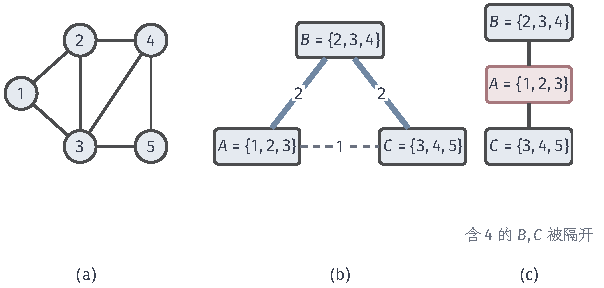
\includegraphics[width=102.306mm]{figures/01-basic-mathematics/04-graphs/tikz/c5-clique-tree-mst/figure.pdf}
  \caption{用交集权重的最大权生成树连接极大团。左：弦图。中：三个极大团组成的候选完全图，边上的数是交集大小，蓝色粗线是总权为$4$的最大权生成树$A-B-C$，虚线是未被选中的候选边。右：总权为$3$的另一棵生成树$B-A-C$，含$4$的团$B,C$被不含$4$的$A$（红色）隔开，不满足运行交集。}
  \label{fig:graph-dp-clique-tree-mst}
\end{figure}

\subsubsection{算法分析}

\paragraph{正确性}
先说明候选集合给出全部极大团。每个$K_v$都是团。反过来，任一团$C$都包含在某个$K_v$中：取$C$中最先被处理的顶点$v$，$C$的其余顶点都在$v$之后且与$v$相邻；沿完美消元序消元不补边也不删去尚未处理的顶点之间的边，它们在处理$v$时仍是$v$的当前邻居，所以都属于$N^+_\pi(v)$。因此每个极大团都等于某个$K_v$（它包含于某个团$K_v$，又是极大的），而不被其他候选严格包含的候选都是极大团。这也说明弦图的极大团数不超过顶点数$n$。

上面的例子中，满足运行交集的树恰好是总权最大的树。下面的定理把思路中的计数写成证明，说明这一对应是一般的。

\begin{theorem}[团树与最大权生成树]
\label{thm:graph-dp-clique-tree-mst}
设$\mathcal H$是非空有限弦图，$\mathcal C$是它的全部极大团。在以$\mathcal C$为顶点的完全图上令$w(C,D)=|C\cap D|$。则一棵生成树满足运行交集，当且仅当它的总权最大。
\end{theorem}

\begin{proof}
先给出任意生成树的总权上界。对生成树$\mathcal T'$，把每条边的权按共享变量拆开计数：
\[
\sum_{\{C,D\}\in\mathcal T'}|C\cap D|=\sum_{v}e_v,
\]
其中$e_v$是两端都含$v$的树边条数。设$v$属于$r_v$个极大团，两端都含$v$的树边正是$\mathcal T'$在这$r_v$个节点上的诱导子图的边；树的诱导子图没有环，是$r_v$个节点上的森林，所以$e_v\leq r_v-1$，且等号成立当且仅当这个诱导子图连通，即含$v$的团在$\mathcal T'$中连通。于是总权不超过$\sum_v(r_v-1)$，等号成立当且仅当对每个$v$都满足运行交集。

剩下要证明确实存在满足运行交集的生成树，即团树存在；那时最大总权恰为$\sum_v(r_v-1)$，最大权生成树就是满足运行交集的生成树。取一个完美消元序，按定理~\ref{thm:graph-dp-elimination-decomposition}的方法以$K_v$为袋得到树分解。若某个袋包含于相邻的袋，就把这条袋树边收缩，只保留较大的袋：顶点覆盖和边覆盖不受影响；对运行交集，被收缩的较小袋中的变量都在较大袋中，收缩一条两端都含$v$的边不破坏$T_v$的连通性，而不含$v$的较小袋本来不在$T_v$中，收缩后$T_v$也不变。

反复收缩，直到没有相邻两袋有包含关系。这时任何两个袋都没有包含关系：若$B_s\subseteq B_t$而$s,t$不相邻，取路径上与$s$相邻的节点$s'$，由运行交集$B_s$的每个变量都在$B_{s'}$中，与“相邻袋无包含关系”矛盾。各袋都是团且互不包含；每个极大团都被某个袋容纳（引理~\ref{lem:graph-dp-clique-in-bag}），而袋本身是团，所以二者相等；每个袋也都是某个极大团，否则它会被那个极大团所在的另一个袋严格包含。于是剩下的袋恰好是全部极大团，各出现一次，团树存在。
\end{proof}

在上例中，$r_1=1$、$r_2=2$、$r_3=3$、$r_4=2$、$r_5=1$，上界$\sum_v(r_v-1)=4$，正好等于$A-B-C$的总权。不连通的弦图中，不同分量的团之间交集为空，零权边只用于把各分量的团树连成一棵树，不影响上界。上面的计数也给出了最后一步核验的做法：检查每个$e_v$是否等于$r_v-1$。

\paragraph{复杂度}
设极大团有$p\leq n$个，候选完全图有$p(p-1)/2$条边，每条边的权需要一次集合求交，排序与并查集的开销按第~\ref{chap:minimum-spanning-tree}章的分析计算。求完美消元序和候选集合的开销见第~\ref{sec:graph-dp-peo-construction}小节与第~\ref{sec:graph-dp-order-to-decomposition}小节。

\paragraph{适用范围}
定理要求输入是弦图，并且使用全部极大团。对无弦四环，极大团是四条边$\{1,2\},\allowbreak\{2,3\},\allowbreak\{3,4\},\allowbreak\{1,4\}$，每个顶点属于两个团；要让每个顶点的两个团相邻，需要四条树边，而四个节点的树只有三条边，所以任何生成树都不满足运行交集。一般图应先弦化，例如用某个消元次序补边，再在弦化后的图上构造团树；在原图的极大团上任选一棵树并不能保证得到树分解。选哪一种弦化决定了袋的大小，而团树构造只负责连接给定弦图的团，不负责找最好的弦化。输出后逐个顶点检查运行交集，也是对输入是否为弦图、团列表是否完整的独立核对。

\subsection{构建结果的检验}
\label{sec:graph-dp-construction-check}

无论结构来自消元次序、贪心规则还是团树构造，交给下一章计算之前都应独立检验。检验只读输出的袋树，不依赖它是怎样构造出来的，所以同样适用于来自别处的分解。检验的对象是原始图$\mathcal G$（有保留集时是$\mathcal G_R$）、局部函数的作用域、袋树及选定的根。

\paragraph{树分解的三个条件}
核验按定义逐条进行：确认袋树是树，即节点数减一等于边数且连通；扫描各袋得到每个顶点的$T_v$，检查顶点覆盖与边覆盖；对每个顶点$v$数出两端袋都含$v$的袋树边条数$e_v$。这些边恰是树在$T_v$上的诱导子图的边，而树的诱导子图是森林，所以$e_v\leq|T_v|-1$，等号成立当且仅当$T_v$连通。

图~\ref{fig:graph-dp-running-intersection}下面的连接中$|T_2|=2$而$e_2=0$，核验失败，$2$就是失败的证据；梯子的分解中$|T_2|=3$、$e_2=2$，通过。团树构造中的最后一步核验（检查每个$e_v$是否等于$r_v-1$）也是这一检查。

\paragraph{作用域、接口与查询}
树分解的条件只涉及原始图的边。计算还需要每个局部函数有处可放，所以对每个作用域$S_a$找出一个包含它的袋并记录下来；引理~\ref{lem:graph-dp-clique-in-bag}保证合法的分解总能通过这项检查，找不到时说明分解本身有误或作用域与原始图不符。

选定根以后，为每个非根节点算出接口$S_u=B_u\cap B_{p(u)}$与内部变量$I_u$，并核对每个变量恰在一个节点作内部变量（引理~\ref{lem:graph-dp-unique-internal}）。有保留集$R$时，另检查根袋包含$R$。最后记录实际宽度，以及各袋、各接口上的状态数之积，供第~\ref{sec:graph-dp-computation-cost}节估计代价。

\paragraph{检验的代价}
设袋树有$N$个节点，各袋大小之和为$L=\sum_t|B_t|$。建立每个顶点的$T_v$和数出各$e_v$需要扫描各袋及各条袋树边两端的公共变量，时间为$O(L+n)$量级（用以变量为下标的数组标记袋内成员）；边覆盖与作用域容纳的检查对每条边或每个作用域，在最小的$T_v$中逐袋测试包含关系。这些都是关于袋大小的多项式开销，与随状态数指数增长的数值计算相比通常很小，但它们是构建阶段的成本，应与构造本身的成本分开记录，不计入下一章的求值时间。

四环算例的分解$\{1,2,4\}-\{2,3,4\}$以$\{2,3,4\}$为根时，检验结果为：四条边分别被两个袋覆盖；$e_2=e_4=1=|T_2|-1=|T_4|-1$，$e_1=e_3=0=|T_1|-1=|T_3|-1$；四个作用域$\{1,2\},\{1,4\}$放进第一个袋，$\{2,3\},\{3,4\}$放进根袋；子节点的接口为$\{2,4\}$、内部变量为$\{1\}$，根的内部变量为$\{2,3,4\}$；宽度为$2$，每个袋上有$8$种配置，接口上有$4$种。

\FloatBarrier
\section{本章小结}
\label{sec:dp-construction-chapter-summary}

本章回答的是：在计算任何数值之前，一般图上的动态规划要把哪些变量放在一起处理、以哪些变量为接口、按什么次序传递结果。构建的输入只是作用域，所得结构对作用域相同而数值任意的全部问题都适用；一般数值下必须保留的耦合一律保留，不利用特定数值的巧合。

合法的结构是原始图的树分解。顶点覆盖和边覆盖保证每个变量、每条边有处可放，而由两两相交子树的公共节点可知，每个作用域乃至每个团都被某个袋整体容纳；运行交集保证每个变量在袋树上占据连成一片的地盘，于是接口把两侧的变量和局部项隔开，以接口为索引的摘要不会丢失信息。选根以后，每个变量恰在它所在的最高节点作内部变量，所以每个变量恰被汇总一次。带保留变量的查询要先把保留集补成团，并选包含它的袋作根，宽度要按补边后的图计算。

变量消元与树分解是同一结构的两种描述。按次序在原始图上模拟消元，填充边记录新产生的耦合，消元簇连到其剩余作用域中最早被消去的变量的袋，就得到树分解，每个非根袋的接口恰是该步中间函数的作用域；反过来，从叶袋向内消去只出现在叶袋中的变量，就读出诱导宽度不超过分解宽度的次序。两个方向合起来，树宽等于最小诱导宽度；但某个具体次序或分解的宽度只是上界，二者也不一一对应。

实际构造时，最小度、最小填充等贪心规则给出可用但不保证最优的次序，状态数不同时还要比较实际的配置数；每个消元次序都隐含一次弦化，弦图有不需补边的完美消元序，可以逐次删除单纯顶点来构造并独立核验；弦图的极大团以交集大小为权、经最大权生成树连成团树。构建结果在交付计算前逐项检验三个条件、作用域容纳、接口与查询根，并记录实际宽度与状态数之积。数值表怎样在这样的结构上计算、怎样恢复配置、代价多大，由下一章回答。

